\documentclass[11pt,fleqn]{report}

\usepackage{latexsym}
\usepackage{makeidx}
\usepackage{amssymb}
%\usepackage{url}
\usepackage{program-text}
\usepackage{color}
\usepackage{a4}
\usepackage{graphicx}
\usepackage{ifthen}
\usepackage[all]{xy}

\input{browseurl}

%%% ------------------------------------------------------------------

\usepackage[colorlinks,linkcolor=blue]{hyperref}
%\usepackage[]{hyperref}
\hypersetup{bookmarksopen=true}
\hypersetup{bookmarksopenlevel=0}
\hypersetup{pdftitle={Curry: A Tutorial Introduction}}
\hypersetup{pdfauthor={S. Antoy and M. Hanus}}
\hypersetup{pdfstartview=FitH}
\usepackage{thumbpdf}

%%% ------------------------------------------------------------------

\setlength{\textwidth}{15.5cm}
\setlength{\textheight}{23cm}
\renewcommand{\baselinestretch}{1.1}
\setlength{\topmargin}{-1cm}
\setlength{\oddsidemargin}{0.5cm}
\setlength{\evensidemargin}{0.5cm}
\setlength{\marginparwidth}{0.0cm}
\setlength{\marginparsep}{0.0cm}

\newlength{\figurewidth}
\setlength{\figurewidth}{\textwidth}
\addtolength{\figurewidth}{-0.4cm}

% base URL for downloading programs:
\def\baseurl{http://www.informatik.uni-kiel.de/~curry/tutorial/}
% reference to a program in the PROGRAMS directory:
\newcommand{\globalproghref}[2]{\href{\baseurl PROGRAMS/#1.pdf}{#2}}
\newcommand{\downloadref}[2]{\href{\baseurl PROGRAMS/chapter\thechapter/#1.curry}{[Download #2]}}

% reference to a program for the current chapter in the PROGRAMS directory:
%\newcommand{\proghref}[2]{\globalproghref{chapter\thechapter/#1}{[#2]}}
\newcommand{\proghref}[2]{\progbrowseurl{chapter\thechapter/#1.curry}{[Browse #2]}\downloadref{#1}{#2}}

\newcommand{\todo}[1]{{\color{red}\sc [{#1}]}}

\newcommand{\pindex}[1]{\index{#1@{\tt #1}}}  % program elements in index

% allow underscores in programs:
\catcode`\_=\active
\let_=\sb
\catcode`\_=12

% ------------------------------------------------------------------
%%% Next should be relative to the current document rather than absolute
%\hyperbaseurl{file:/home/mh/papers/tutorial/}
\newtheorem{rmexercise}{Exercise}
\newenvironment{exercise}{\begin{rmexercise}\rm}{\end{rmexercise}}
% ------------------------------------------------------------------

% ------------------------------------------------------------------
\newcommand{\curryurl}{http://www.curry-language.org}
\newcommand{\curry}%
  {\href{\curryurl}{Curry}}
\newcommand{\pakcs}%
  {\href{http://www.informatik.uni-kiel.de/~pakcs}{{\sc PAKCS}}}
\newcommand{\wwwc}{\href{http://www.w3c.org}{W3C}}
% ------------------------------------------------------------------

% produce an index:
\makeindex

\begin{document}
\sloppy

\pagenumbering{roman}
\begin{titlepage}
\begin{center}
\fbox{
\begin{minipage}[t]{\figurewidth}
\begin{center}\vspace{20ex}
{\Huge\bf Curry}\\[4ex]
{\LARGE\bf A Tutorial Introduction}\\[5ex]
{\large Draft of \today}\\[8ex]
\Large
\href{http://www.cs.pdx.edu/~antoy/}{Sergio Antoy}\\[1ex]
\large
\href{http://www.pdx.edu}{Portland State University}, U.S.A.\\
Web: \url{http://www.cs.pdx.edu/~antoy/}\\[3ex]
\Large
\href{http://www.informatik.uni-kiel.de/~mh/}{Michael Hanus}\\[1ex]
\large
\href{http://www.uni-kiel.de}{Christian-Albrechts-Universit\"at Kiel}, Germany\\
Web: \url{http://www.informatik.uni-kiel.de/~mh/}\\
\vspace{20ex}
\end{center}
\end{minipage}}
\end{center}
\setcounter{page}{0} 
\end{titlepage}
\pdfbookmark[1]{Contents}{Contents}
\tableofcontents

\newpage
\pagenumbering{arabic}

\chapter*{Preface}
\addcontentsline{toc}{chapter}{Preface}

This book is about programming in \curry,
a general-purpose declarative programming language
that integrates functional with logic programming.
Curry seamlessly combines the key features of
functional programming (nested expressions, lazy evaluation,
higher-order functions), logic programming (logical variables,
partial data structures, built-in search), and concurrent
programming (concurrent evaluation of constraints with synchronization
on logical variables).

This book is best used as an introduction to Curry.
Curry is a rigorously defined programming language.
The \href{\curryurl/documentation/report}
{``Report''} is a still evolving, but fairly stable,
document that precisely defines the language,
in particular both its syntax and operational semantics.
However, the report is not best suited to the beginner,
rather it may be consulted in conjunction with this
tutorial for the sake of a completeness that is not sought here.

There are several
\href{\curryurl/implementations/overview}{implementations of Curry}.
%The most usable at the time of the writing (July~2014) is \pakcs.
The examples and exercises in this book have been developed
and executed using \pakcs.
PAKCS is also accessible (in a restricted form) on-line via a
\href{http://www-ps.informatik.uni-kiel.de/smap/}{web-based system}.
In this document, you find for many programs a ``Browse'' link
which directly loads the program into this web-based system so that
you can run or modify it.
Alternatively, you can download the example programs
and execute them on your locally installed Curry system.

% Numerous people have contributed directly and indirectly to Curry.
% We are grateful to the following people for 
% discussions, comments and suggestions: ...


\part{Language Features}
\chapter{Introduction}

Curry is a universal programming language aiming at the amalgamation
of the most important declarative programming paradigms,
namely functional programming and logic programming.  
Curry combines in a seamless way features from functional programming
(nested expressions, lazy evaluation, higher-order functions),
logic programming (logical variables, partial data structures,
built-in search), and concurrent programming (concurrent evaluation
of constraints with synchronization on logical variables).
Moreover, Curry provides additional features in
comparison to the pure languages (compared to functional programming:
search, computing with partial information; compared to logic
programming: more efficient evaluation due to the deterministic
evaluation of functions).
Moreover, it also amalgamates the most
important operational principles developed in the area of integrated
functional logic languages: ``residuation'' and ``narrowing'' (see
\cite{Hanus94JLP,Hanus07ICLP} for surveys on functional logic programming).

The development of Curry is an international initiative intended to
provide a common platform for the research, teaching\footnote{%
Actually, Curry has been successfully applied to teach functional and
logic programming techniques in a single course without switching
between different programming languages. More details about
this aspect can be found in \cite{Hanus97DPLE}.}
and application of integrated functional logic languages.

This document is intended to provide a tutorial introduction
into the features of Curry and their use in application programming.
It is not a formal definition of Curry which can be found
in \cite{Hanus16Curry}.

%\todo{Update and complete this chapter.}



%%% Local Variables: 
%%% mode: latex
%%% TeX-master: "main"
%%% End: 

\chapter{Getting Started with Curry}

There are different implementations of \curry{}
available\footnote{Check the web page \url{\curryurl} for details.}.
As such we can not describe the use of a Curry system
in general. Some implementations are batch-oriented.  In this case a 
Curry program is compiled into machine code and then executed. 
In this introduction we prefer an implementation that supports an interactive environment which provides faster program development by loading and testing programs within the integrated environment.

\pakcs\index{PAKCS} (Portland Aachen Kiel Curry System)
\cite{Hanus14PAKCS}\footnote{\url{http://www.informatik.uni-kiel.de/~pakcs}}
contains such an interactive environment so that we show the use
of this system here in order to get started with Curry.
When you start the interactive environment of PAKCS
(e.g., by typing \ccode{pakcs}\pindex{pakcs}
as a shell command),
you see something like the following output after the system's
initialization:
\begin{verbatim}
     ______      __       _    _    ______   _______     
    |  __  |    /  \     | |  / /  |  ____| |  _____|   Portland Aachen Kiel
    | |  | |   / /\ \    | |_/ /   | |      | |_____    Curry System
    | |__| |  / /__\ \   |  _  |   | |      |_____  |   
    |  ____| / ______ \  | | \ \   | |____   _____| |   Version 1.11.3 (1)
    |_|     /_/      \_\ |_|  \_\  |______| |_______|   
   
   Curry2Prolog(sicstus 4.2) Compiler Environment (Version of 2014-07-21)
   (RWTH Aachen, CAU Kiel, Portland State University)
   
   Type ":h" for help (contact: pakcs@curry-language.org)
   Prelude> 
\end{verbatim}
Now the system is ready and waits for some input.
By typing \ccode{:q} (quit) you can always leave the system,
but this is not what we intend to do now.
The prefix of the current input line always shows the currently
loaded module or program. In this case the module
\code{Prelude}\pindex{Prelude}
is loaded during system startup.
The standard system module \code{Prelude} contains
the definition of several predefined functions and data structures
which are available in all Curry programs.
For instance, the standard arithmetic functions like \code{+}, \code{*} etc
are predefined so that we can use the system as a simple calculator
(the input typed by the user is underlined):
\begin{prog}
Prelude> \userinput{3+5*4}
23
\end{prog}
In this simple example you can already see the basic functionality
of the environment: if you type an expression, the system
evaluates this expression to a \emph{value}\index{value}
(i.e., an expression without evaluable functions)
and prints this value as the result. % (with a question mark, see below).
%Now hit the ``enter'' key and you are back to input line mode where
Now you can type additional expressions to be evaluated. For instance,
you can compare the values of two expressions with the
usual comparison operators \code{>}, \code{<}, \code{<=}, \code{>=}:
\begin{prog}
Prelude> \userinput{3+5*4 >= 3*(4+2)}
True
\end{prog}
\code{==} and \code{/=} are the operators for equality and disequality
and can be used on numbers as well as on other datatypes:
\begin{prog}
Prelude> \userinput{4+3 == 8}
False
\end{prog}
% You may wonder why the system always puts a question mark after
% the result and then waits for further input.
% The reason is that Curry cannot only perform functional, thus,
% purely deterministic computations, which yields at most one result;
% Curry subsumes logic languages which are able
% to search for different results. Therefore, arbitrary
% expressions might deliver several solutions and PAKCS
% computes these solutions one after the other. Thus, it prints
% the first solution followed by a question mark and,
% if you type \ccode{;} (followed by
% the ``enter'' key), it computes and prints the next solution and so on.
% We will see later examples for this feature but ignore it
% for the moment. So, just hit the ``enter'' key after a result
% in order to ignore the computation of further solutions.
% 
One may want to use Curry as more than a mere desk calculator. Therefore, we will discuss how to write programs in Curry.
In general, a Curry \emph{program}\index{program}
is a set of function definitions.
The simplest sort of functions are those that do not depend
on any input value, i.e., constant functions.
For instance, a definition like
\begin{prog}
nine = 3*3
\end{prog}
(such definitions are also called \emph{rules}\index{rule}
or \emph{defining equations}\index{defining equation}\index{equation!defining})
defines the name \code{nine} as equal to the value of \code{3*3},
i.e., \code{9}. This means that each occurrence of the name \code{nine}
in an expression is replaced by the value \code{9}, i.e., the value
of the expression \ccode{4*nine} is \code{36}.

Of course, it is more interesting to define functions depending
on some input arguments. For instance, a function to compute the
square value of a given number can be defined by
\begin{prog}
square x = x*x
\end{prog}
Now it is time to make some remarks about the syntax
of Curry (which is actually very similar to
Haskell \cite{PeytonJones03Haskell}).
The names of functions and parameters usually start with
a lowercase letter followed by letters, digits and underscores.
The application of a function $f$ to an expression $e$ is denoted
by juxtaposition, i.e., by ``$f~e$''. An exception are the
\emph{infix operators}%
\index{operator}\index{operator!infix}\index{infix operator}
like \code{+} or \code{*} that can be written between
their arguments to enable the standard mathematical notation
for arithmetic expressions. Furthermore, these operators
are defined with the usual associativity and precedence rules
so that an expression like \ccode{2+3+4*5} is interpreted
as \code{((2+3)+(4*5))}. However, one can also enclose
expressions in parenthesis to enforce the intended grouping.

If we write the definitions of \code{nine} and \code{square}
with a standard text editor
into a file (note that each definition must be written on a separate
line starting in the first column) named \ccode{firstprog.curry}
(\proghref{firstprog}{Program}),
we can load (and compile) the program into our environment
by the command
\begin{prog}
Prelude> \userinput{:l firstprog}
\end{prog}
which reads and compiles the file \ccode{firstprog.curry} and
makes all definitions in this program visible in the environment.
After the successful processing of this program, the environment
shows the prefix to the input line as
\begin{prog}
firstprog>
\end{prog}
indicating that the program \ccode{firstprog} is currently loaded.
Now we can use the definitions in this program in the expressions
to be evaluated:
\begin{prog}
firstprog> \userinput{square nine}
81
\end{prog}
If we change our currently loaded program, we can easily reload
the new version by typing \ccode{:r}. For instance,
if we add the definition \ccode{two = 2} to our file
\ccode{firstprog.curry}, we can reload the program as follows:
\begin{prog}
firstprog> \userinput{:r}
\ldots
firstprog> \userinput{square (square two)}
16
\end{prog}
Functions containing only a single arithmetic expression in the
right-hand side of their defining equations might be useful abstractions
of complex expressions but are generally only of limited use.
More interesting functions can be written using conditional
expressions. A \emph{conditional expression}%
\index{conditional expression}\index{expression!conditional}
has the general form \ccode{if $c$ then $e_1$ else $e_2$}
where $c$ is a Boolean expression (yielding the value \code{True}
or \code{False}). A conditional expression is evaluated by
evaluating the condition $c$ first. If its value is \code{True},
the value of the conditional is the value of $e_1$, otherwise
it is the value of $e_2$. For instance, the following rule
defines a function to compute the absolute value of a number:
\begin{prog}
abs x = if x>=0 then x else -x
\end{prog}
Using recursive definitions, i.e., rules where the defined
function occurs in a recursive call in the right-hand side,
we can define functions whose evaluation requires a non-constant
number of evaluation steps. For instance, the following rule
defines the factorial of a natural number
\proghref{absfac}{Program}:
\begin{prog}
fac n = if n==0 then 1
                else n * fac(n-1)
\end{prog}
Note that function definitions can be put in several lines
provided that the subsequent lines start in a column greater
than the column where the left-hand side starts
(this is also called the \emph{layout}\index{layout rule}
or \emph{off-side}\index{off-side rule} rule for separating
definitions).

You might have noticed that functions are defined by rules
like in mathematics without providing any type declarations.
This does not mean that Curry is an untyped language.  On the contrary, Curry is a \emph{strongly typed language}\index{types}
which means that each entity in a program (e.g., functions, parameters)
has a type and ill-typed combinations are detected
by the compiler. For instance, expressions like
\ccode{3*True} or \ccode{fac False} are rejected by the compiler.
Although type annotations need not be written by the programmer,
they are automatically inferred by the compiler
using a \emph{type inference algorithm}\index{type inference}.
Nevertheless, it is a good idea to write down the types
of functions in order to provide at least a minimal documentation
of the intended use of functions. For instance,
the function \code{fac} maps integers into integers and so
its type can be specified by
\begin{prog}
fac :: Int -> Int
\end{prog}
(\code{Int} denotes the predefined type of integers; similarly
\code{Bool} denotes the type of Boolean values).
If one is interested in the type of a function or expression
inferred by the type inference algorithm, one can show it
using the command \ccode{:t} in PAKCS:
\begin{prog}
absfac> \userinput{:t fac}
fac :: Int -> Int
absfac> \userinput{:t  abs 3}
(abs 3) :: Int
\end{prog}
%
A useful feature of Curry (as well as most functional and logic
programming languages) is the ability to define
functions in a \emph{pattern-oriented style}.\index{pattern}
This means that we can put values like \code{True} or \code{False}
in arguments of the left-hand side of a rule
and define a function by using several rules.  The rule that matches the pattern of left-hand side will be called.   
For instance, instead of defining the negation on Boolean values by
the single rule
\begin{prog}
not x = if x==True then False
                   else True
\end{prog}
we can define it by using two rules, each with a different pattern (here we
also add the type declaration):
\begin{prog}
not :: Bool -> Bool
not False = True
not True  = False
\end{prog}
The pattern-oriented notation becomes very useful in combination
with more complex data structures, as we will see later.

One of the distinguishing features of Curry in comparison
to functional languages is its ability to \emph{search for solutions},
i.e., to compute values for the arguments of functions so that
the functions can be evaluated.
For instance, consider the following definitions of some functions
on Boolean values contained in the prelude (note that
Curry also allows functions defined as infix operators, i.e.,
\ccode{x \&\& y} denotes the application of function \code{\&\&}
to the arguments \code{x} and \code{y}):
\begin{prog}
False \&\& _  =  False
True  \&\& x  =  x
~
False || x  =  x
True  || _  =  True
~
not False   =  True
not True    =  False
\end{prog}
The underscore
\ccode{_}\pindex{_}\index{variable!anonymous}\index{anonymous variable}
occurring in the rules for
\code{\&\&} and \code{||} denotes an arbitrary value,
i.e., such an \emph{anonymous variable} is used for argument
variables that occur only once in a rule.

We can use these definitions to compute the value of a Boolean expression:
\begin{prog}
Prelude> \userinput{True \&\& (True || (not True))}
True
\end{prog}
However, we can do more and use the same functions
to compute Boolean values for some (initially unknown) arguments:
\begin{prog}
Prelude> \userinput{x \&\& (y || (not x))  where x,y free}
\{x=True, y=True\} True
\{x=True, y=False\} False
\{x=False, y=y\} False
\end{prog}
Note that the initial expression contains the
\emph{free variables}\index{free variable}\index{variable!free}
\code{x} and \code{y} as arguments.
To support the detection of typos,
free variables in initial expressions must be explicitly declared
by a \ccode{where\ldots{}free} clause at the end of the expression.
This requirement can be relaxed in PAKCS by turning the
\emph{free variable mode} on by the command \ccode{:set +free}.
In this mode, all identifiers in the initial expression that
are not defined in the currently loaded program are considered as
free variables:
\begin{prog}
Prelude> \userinput{:set +free}
Prelude> \userinput{x \&\& (y || (not x))}
\{x=True, y=True\} True
\{x=True, y=False\} False
\{x=False, y=y\} False
\end{prog}
Free variables denote ``unknown'' values.
They are instantiated (i.e., replaced by some concrete values) so that
the instantiated expression is evaluable. As we have seen above,
replacing both \code{x} and \code{y} by \code{True}
makes the expression reducible to \code{True}. Therefore,
the Curry system shows in the first result line \code{True} together with the
bindings (i.e., instantiations) of the free variables
it has done to compute this value.

In general, there is more than one possibility
to instantiate the arguments, e.g., the Boolean variables
\code{x} and \code{y} can be instantiated to \code{True} or \code{False}.
This leads to different solutions which are printed
one after the other as shown above: there is one instantiation
for \code{x} and \code{y} so that the instantiated expression
evaluates to \code{True}, and there are two instantiations
so that the instantiated expression evaluates to \code{False}.
The last result line shows that the initial expression has the value
\code{False} provided that \code{x} is instantiated to \code{False}
but \code{y} can be arbitrary (i.e., \code{y} is not instantiated).

As we have seen, PAKCS evaluates and shows all the values
(also called solutions if variables are instantiated)
of an initial expression. This default mode can be changed
by the command \ccode{:set +interactive}.
In the \emph{interactive mode}, we are asked after each
computed value how to proceed:
whether we want to see the next value (``yes''), no more values (``no''),
or all values without any further interaction (``all'').
Thus, we can show the values of the initial expression
step-by-step as follows (note that it is sufficient to type
the first letter of the answer followed by the ``enter'' key):
\begin{prog}
Prelude> \userinput{:set +interactive}
Prelude> \userinput{x \&\& (y || (not x))  where x,y free}
\{x=True, y=True\}  True
More values? [Y(es)/n(o)/a(ll)] \userinput{y}
\{x=True, y=False\} False
More values? [Y(es)/n(o)/a(ll)] \userinput{y}
\{x=False, y=y\} False
More values? [Y(es)/n(o)/a(ll)] \userinput{y}
No more values.
\end{prog}
The final line indicates that there are no more values to the
initial expression. This situation can also occur if functions
are partially defined, i.e., there is a call to which no rule
is applicable. For instance, assume that we define the function
\code{pneg} by the single rule
\proghref{bool}{Program}
\begin{prog}
pneg True = False
\end{prog}
then there is no rule to evaluate the call \ccode{pneg False}:
\begin{prog}
bool> \userinput{pneg False}
No more values.
\end{prog}
As we have seen in the Boolean example above,
Curry can evaluate expressions containing free variables
by guessing values for the free variables so that the expression
becomes evaluable (the concrete strategy used by Curry will be
explained later, but don't worry: Curry is based on an optimal
evaluation strategy \cite{AntoyEchahedHanus00JACM} that performs
these instantiations in a goal-oriented manner).
However, we might not be interested to see
all possible evaluations but only those that lead to a required
result. For instance, we might be only interested to compute
instantiations in a Boolean formula so that the formula becomes true,
e.g., as in solving an equation.

For this purpose, Curry offers \emph{constraints}\index{constraint},
i.e., formulas that are intended to be solved (instead of computing
an overall value). One of the basic constraints supported by Curry
is equality, i.e., \ccode{$e_1$ =:= $e_2$} denotes an
\emph{equational constraint}\index{equational constraint}%
\index{constraint!equational}
which is solvable whenever the expressions $e_1$ and $e_2$
(which must be of the same type) can be instantiated so that
they are evaluable to the same value. For instance,
the constraint \ccode{1+4=:=5} is solvable, and
the constraint \ccode{2+3=:=x} is solvable if the variable \code{x}
is instantiated to \code{5}. Now we can compute positive solutions
to a Boolean expression by solving a constraint containing \code{True}
on one side:
\begin{prog}
Prelude> \userinput{(x \&\& (y || (not x))) =:= True  where x,y free}
\{x=True, y=True\} True
\end{prog}
% Note that \ccode{success}\pindex{success}
% denotes the trivial, always satisfiable
% constraint, i.e., a result like \ccode{success} indicates that
% the constraint is satisfied with respect to the computed instantiations.
Curry allows the definition of functions by several rules
and is able to search for several solutions. We can combine
both features to define functions that yield more than one
result for a given input. Such functions are called
\emph{non-deterministic} or \emph{set-valued functions}.%
\index{function!non-deterministic}\index{non-deterministic function}%
\index{function!set-valued}\index{set-valued function}
A simple example for a set-valued function
is the following function \code{choose} which yields
non-deterministically one of its arguments as a result
\proghref{choose}{Program}:
\begin{prog}
choose x y = x
choose x y = y
\end{prog}
With this function we could have several results for a particular call:
\begin{prog}
choose> \userinput{choose 1 3}
1
3
\end{prog}
We can use \code{choose} to define other set-valued functions:
\begin{prog}
one23 = choose 1 (choose 2 3)
\end{prog}
Thus, a call to \code{one23} delivers one of the results \code{1},
\code{2}, or \code{3}. Such a function might be useful
to specify the domain of values for which we want to solve a
constraint. For instance, to search for values $x \in \{1,2,3\}$
satisfying the equation $x+x = x*x$, we can solve
this constraint ($c_1\,\code{\&}\,c_2$ denotes the conjunction
of the two constraints $c_1$ and $c_2$):
\begin{prog}
choose> \userinput{x=:=one23 \& x+x=:=x*x  where x free}
\{x=2\} True
\end{prog}
Set-valued functions are often a reasonable alternative
to flexible functions in order to search for solutions.
The advantages of set-valued functions will become clear
when we have discussed the (demand-driven) evaluation strategy
in more detail.

This chapter is intended to provide a broad overview
of the main features of Curry and the use of an interactive
programming environment so that one can easily try the subsequent
examples. In the next chapter, we will discuss the features
of Curry in more detail.


%%% Local Variables: 
%%% mode: latex
%%% TeX-master: "main"
%%% End: 

\chapter{Main Features of Curry}

\section{Overview}

The major elements declared in program are
\emph{functions} and \emph{data structures}.

\begin{itemize}
\item{} 
A \define{function} or \define{operation} defines
a computation similar to an expression.
However, the expression computed by a function
has a name and is often parameterized.
These characteristics enable you to execute the same computation, possibly
with different parameters, over and over in the same program
by simply invoking the computation's name
and setting the values of its parameters.
A function also provides a \emph{procedural abstraction}.
Rather than coding a computation by means of a possibly
complicated expression, you can factor out portions of this computation
and abstract them by their names.
\item{} 
A \define{data structure} is a way to organize data.
For example, you can record the movements of your bank account
in a column in which deposits are positive numbers and withdrawals
are negative numbers.  Or you can record the same movements in
two columns, one for deposits and another for withdrawals,
in which all numbers are positive.
With the second option,
the columns rather than the signs specialize the meaning of the numbers.
The way in which information is organized may ease some computations,
such as retrieving portions of information, and
is intimately related, through pattern matching,
to the way in which functions are coded.
\end{itemize}
%
This section describes in some detail both of these features and
a number of related concepts.
Curry has some additional features not described in this section.
Since they are useful to support particular programming tasks,
we introduce them later when we discuss such programming techniques.


\section{Expressions}

A function can be regarded as a parameterized expression with a name.
Thus, we begin by explaining what an expression is and
how it is used.
Most expressions are built from simpler subexpressions,
a situation that calls for a recursive, or inductive, definition.
%
\begin{quote}
An \definei{expression}{expression!definition}
is either a symbol or literal value or
is the application of an expression to another expression.
\end{quote}
%
A symbol or literal value is referred to as an \emph{atom}\index{atom}.
For example, numbers and the Boolean symbols \ccode{True}
and \ccode{False} are examples of atoms.
Atoms constitute the most elementary expressions.
These elementary expressions can be combined to create
more complex expressions, e.g., \ccode{2\,+\,3} or
\ccode{not\,\,True}.
The combination is referred to as a
\emph{function application}\index{function!application}.
Since a function application is a very common activity,
it is convenient to denote it as simply as possible.
This convenience is obtained to the extreme by writing the two expressions one
near the other as in \ccode{not\,\,True}.
This notation is referred to as \emph{juxtaposition}\index{juxtaposition}.

In the above expressions, the symbols \ccode{+} and
\ccode{not} are operations.
Both are predefined in the standard library \code{Prelude}\pindex{Prelude}.
Although conceptually the symbols \ccode{+} and \ccode{not}
are alike, syntactically they differ.
The symbol \ccode{+} is a \emph{infix operator}
as in the ordinary mathematical notation.  
Infix operators have a \emph{precedence}\index{infix operator!precedence}
and an \emph{associativity}\index{infix operator!associativity}
so that the expression \ccode{2\,+\,3\,*\,4}
is understood as \ccode{2\,+\,(3\,*\,4)} and
the expression \ccode{4\,-\,3\,-\,2} is understood
as \ccode{(4\,-\,3)\,-\,2}.
The precedence and associativity of an infix symbol
are defined in a program by a declaration.
The following declarations, from the prelude,
define these parameters for some ordinary arithmetic operations:
%
\begin{curry}
infixl 7 *, `div`, `mod`
infixl 6 +, -
infix  4  <, >, <=, >=
\end{curry}
%
For example, 
the precedence of the addition and subtraction operators is 6
and their associativity is left.
The relational operators have precedence 4 and are not associative.
Operators with a higher precedence bind stronger, i.e.,
the expression \ccode{4\,<\,2\,+\,3} is interpreted as
\ccode{4\,<\,(2\,+\,3)}.\index{infix operator!precedence}
%
\begin{quote}
\emph{Infix declarations}\index{infix operator!declaration}
must always occur at the beginning of a program.
The precedence of an operator\index{precedence!values}
is an integer between 0 and 9 inclusive.
The associativity of an operator\index{associativity!values} is either
\emph{left}, denoted by the keyword \ccode{infixl}\pindex{infixl}
or \emph{right}, denoted by the keyword \ccode{infixr}\pindex{infixr}.
Non-associative infix operators are declared using the 
keyword \ccode{infix}\pindex{infix}.
\end{quote}
%
Most often, an infix operator is any user-defined sequence of characters
taken from the set
``\verb`~!@#$%^&*+-=<>?./|\:`''\index{infix operator!character set}.
% $ to balance groups
Alphanumeric identifiers can be defined and used as infix operators
if they are surrounded by backquotes, as \ccode{`div`} and
\ccode{`mod`} in the previous declaration.
For example, for any integer value $x$, the following expression
evaluates to $x$ itself.
%
\begin{prog}
$x$ `div` 2 * 2 + $x$ `mod` 2
\end{prog}
%
Non-infix symbols are \emph{prefix}\index{prefix}.
They are applied by prefixing them to their arguments as in
\ccode{not\,\,True}.

\begin{exercise}
\label{ex_factor}
Define a predicate, read as ``factors'' and denoted by
the infix operator ``\verb|./.|'', that tells whether an
integer is a factor of another integer.
The predicate should work for every input and \code{0}
should not be a factor of any integer.
The operator should be non-associative and have precedence 7.
\proghref{exfactor}{Answer}
\end{exercise}

A symbol, whether infix or prefix, can only be applied to
values of an appropriate type.
As one would expect, the Boolean negation operator can be
applied only to a Boolean value.
For example, the expression \ccode{not\,\,2} is an error.
The compiler/interpreter would
report that the expression is incorrectly typed.
We will discuss types in more detail after presenting
data declarations.

The application of an expression to another is a binary operation.
The expression that is being applied is referred to as the
\emph{function} of the application.
The other expression is referred to as the \emph{argument}.
Thus, in \ccode{not\,\,True}, \ccode{not} is the function
and \ccode{True} is the argument.
The situation is slightly more complicated for infix operations.
The reading of \ccode{2\,+\,3} is that the function \ccode{+}
is applied to the expression \ccode{2}.
The result is a function which is further applied to the expression
\ccode{3}.

Expressions can also be conditional, i.e., depend
on the value of a Boolean expression.
Such \emph{conditional expressions}%
\index{conditional expression}\index{expression!conditional}%
\pindex{if-then-else}
have the form \ccode{if $b$ then $e_1$ else $e_2$}.
The value of this expression is the value of $e_1$ if $b$ evaluates
to \code{True}, or the value of $e_2$ if $b$ evaluates to \code{False}.
Thus, the value of \ccode{if 3>4 then 2*2 else 3*4} is \code{12}.


\section{Predefined Types}
\label{Predefined Types}

A \emph{type}\index{type} is a set of values.
Ubiquitous types, such as integers or characters,
are predefined by most programming languages.
Curry makes no exception.
These types are referred to as \emph{builtin}\index{type!builtin}
and are denoted with a familiar, somewhat special, syntax.
Both the availability of builtin types and their characteristics
may depend on a specific implementation of Curry.
The following table summarizes some types available in \pakcs.
%
\begin{center}
\begin{tabular}{@{} || l | l | l || @{}}
\hline \hline
\bf Type & \bf Declaration & \bf Examples \\
\hline
\hline
Integer & \code{Int} & \verb|...,-2,-1,0,1,2,...| \\
\hline
Boolean & \code{Bool} & \code{False, True} \\
\hline
Character & \code{Char} & \verb|'a','b','c',...,'\n',...| \\
\hline
String & \code{String} & \code{"hello", "world"} \\
\hline
List of $\tau$ & \code{[$\tau$]} & \code{[], [0,1,2], 0:1:2:[]} \\
\hline
Unit & \code{()} & \code{()} \\
\hline \hline
\end{tabular}
\end{center}
\pindex{Int}\pindex{Bool}\pindex{Char}%
\pindex{String}\index{List}\index{unit type}\pindex{()}
%
The details of these types are found in the {\pakcs} User Manual.
Below, we only outline a few crucial characteristics of the builtin types.
The integers have arbitrary precision.
Some frequently used non-printable characters are denoted,
as in other popular programming languages,
by escape sequences, e.g., \emph{newline} is denoted by \verb|\n|.
The type \emph{List}\index{list} represents sequences of values.
This type is polymorphic, i.e.,
for any type $\tau$, the type list of $\tau$,
denoted by \ccode{[$\tau$]}, is a type whose instances
are sequences of instances of $\tau$.
The last two examples in the \emph{List} row of the table
denote a list of integers,
their type denoted by \ccode{[Int]}.
The notation of lists will be further discussed later.
The symbol \ccode{()}\pindex{()} denotes the unit type as well as the only
element of this type. The unit type is useful in situations
where the return value of a function is not important.
Another useful type available in {\pakcs},
the \emph{tuple}\index{tuple}, will be described later.


\section{Predefined Operations}
\label{Predefined Operations}

Many frequently-used functions and infix operators,
similar to frequently-used types, are predefined in Curry.
Some of these can be found in the \ccode{Prelude},
a Curry source program automatically loaded when the
compiler/interpreter starts.
A few others are so fundamental that they are built into the language.
Some of these functions and operators are shown in the following table.
%
\begin{center}
\begin{tabular}{@{} || l | c | c | c | l || @{}}
\hline \hline
\bf Description & \bf Ident. & \bf Fix. & \bf Prec. & \bf Type \\
\hline \hline
Boolean equality & {\tt ==} & & 4 & {\tt a -> a -> Bool} \\
\hline
Constrained equality & {\tt =:=} & & 4 & {\tt a -> a -> Bool} \\
\hline
Boolean conjunction & {\tt \&\&} & R & 3 & {\tt Bool -> Bool -> Bool} \\
\hline
Boolean disjunction & {\tt ||} & R & 2 & {\tt Bool -> Bool -> Bool} \\
\hline
Parallel conjunction & {\tt \&} & R & 0 & {\tt Bool -> Bool -> Bool} \\
\hline
Constrained expression & {\tt \&>} & R & 0 & {\tt Bool -> a -> a} \\
\hline
\hline
\end{tabular}
\end{center}
\pindex{==}\pindex{=:=}\pindex{\&\&}\pindex{\char124\char124}\pindex{\&}\pindex{\&>}

\vspace{3ex}
\noindent
Because of non-determinism and free variables, in the following discussion,
different evaluations of the same expression may produce different values.
\\[1ex]
The \emph{Boolean equality}\index{Boolean equality}\index{equality!Boolean}
applied to expressions $u$ and $v$, i.e.,
$u\;\mbox{\tt ==}\;v$, returns \ccode{True}
when $u$ and $v$ evaluate to the
same \emph{value} and \ccode{False} when they
evaluate to different \emph{values}---a
more precise definition will be given later. 
If the evaluation of $u$ and/or $v$ ends in an expression that
still contains functions, e.g., \code{1 `div` 0}, the computation
\emph{fails} and no value is returned.
\\[1ex]
The \emph{constrained equality}\index{constrained equality}%
\index{equality!constrained}
applied to expressions $u$ and $v$, i.e.,
$u\;\mbox{\tt =:=}\;v$ returns \ccode{True}
when $u$ and $v$ evaluate to the
same \emph{value}---a precise definition will be given later. 
Otherwise, the computation \emph{fails} and no value is returned.
A key difference between the Boolean and the constrained equalities
is how they evaluate expressions containing variables.
This will be discussed in some detail in Section~\ref{Logic variables}.
\\[1ex]
The \emph{Boolean conjunction}\index{Boolean conjunction}%
\index{conjunction!Boolean}
applied to expressions $u$ and $v$, i.e.,
$u\;\mbox{\tt \&\&}\;v$, returns \ccode{True}
when $u$ and $v$ evaluate to \ccode{True}.
\\[1ex]
The \emph{Boolean disjunction}\index{Boolean disjunction}%
\index{disjunction!Boolean}
applied to expressions $u$ and $v$, i.e.,
$u\;\mbox{\tt ||}\;v$, returns \ccode{True}
when $u$ or $v$ evaluate to \ccode{True}.
\\[1ex]
The \emph{parallel conjunction}\index{parallel conjunction}%
\index{conjunction!parallel}
applied to expressions $u$ and $v$, i.e.,
$u\;\mbox{\tt \&}\;v$, evaluates $u$ and $v$ concurrently.
If both succeeds, the evaluation succeeds;
otherwise it fails.
\\[1ex]
The \emph{constrained expression}\index{constrained expression}%
\index{expression!constrained}
applied to a constraint $c$ and an expression $e$, i.e.,
$c\;\mbox{\tt \&>}\;e$, evaluates first $c$ and, if $c$ evaluates
to \ccode{True}, then the result is the value of $e$, otherwise it fails.

Curry predefines many more functions and operations, e.g.,
the standard arithmetic and relational operators on numbers.
A complete list can be found both in the Report and the \ccode{Prelude}.

\section{Functions}

\subsection{Basic Concepts}
\label{Basic concepts}

A program function abstracts a function in the mathematical sense.
A function is a device that takes arguments and returns a result.
The result is obtained by evaluating an expression
which generally involves the function's arguments.
The following function computes the \emph{square} of a number.
%
\begin{curry}
square x = x * x
\end{curry}
%
The symbols \ccode{square} is the name or
\emph{identifier}\index{function!identifier} of the function.
The symbol \ccode{x} is the function's 
\emph{argument}\index{function!argument}.
The above declaration is referred to as a
\emph{rewrite rule}\index{rewrite rule}, or simply a rule,
defining a function.
The portion of the declaration to the left of the symbol \ccode{=}
is the rule's \emph{left-hand side}\index{rewrite rule!left-hand side}.
The expression \ccode{x\,*\,x} is the rule's
\emph{right-hand side}\index{rewrite rule!right-hand side}.

When the \ccode{square} symbol is applied to an expression,
e.g., \ccode{2\,+\,3}, this expression is
\emph{bound}\index{function!argument binding}
to the argument \ccode{x}.
The result of the application is
\ccode{(2\,+\,3)\,*\,(2\,+\,3)}, i.e., the body
in which the argument is replaced by its binding.
Thus:
%
\begin{prog}
Prelude> \userinput{square (2+3)}
25
\end{prog}
%
Functions can be \emph{anonymous}\index{function!anonymous},
i.e., without a name.
An anonymous function is useful when a function is referenced
only once.  In this case, the reference to the function
can be replaced by the expression defining the function.
In the following example:
%
\begin{curry}
result = (\x -> x * x) (2+3)
\end{curry}
%
the value of \code{result} is \code{25}.
It is obtained by applying the expression
\code{(\char92x -> x * x)}, an anonymous function,
to \code{(2+3)}, its argument.
An anonymous function definition has the following structure:
%
\begin{curry}
\ <arguments> -> <right-hand side>
\end{curry}
%
The arguments are listed as in any rewrite rule.
The right-hand side is the expression to be evaluated
when the anonymous function is applied to actual arguments.
A more motivating example of anonymous function
is presented in Section~\ref{Higher-Order}

The evaluation\index{evaluation} of any expression,
in particular of a function application,
is \emph{lazy}\index{evaluation!lazy}.
This means that the computation of any expression,
including the subexpressions of a larger expression,
is delayed until the expression's value is actually needed.
The exact meaning of ``actually needed'' is quite technical,
but the intuitive meaning suffices for our purposes.
Many programming languages, such as C and Java,
adopt this evaluation strategy, under the name of
\emph{short circuit}\index{evaluation!short circuit},
only for Boolean expressions.

We will discuss this issue in more detail later.
Although the lazy evaluation strategy is conceptually simpler
than any other strategy, many traditional programming languages
evaluate the arguments of a function call eagerly, i.e.,
before applying a function to its arguments.
This fact is sometimes a source of confusion for the beginner.

\subsection{Pattern Matching}
\label{Pattern Matching}

The definition of a function can be broken into several
rules\index{rewrite rule}.
A single rule would suffice in many cases.
However, several rules allows a definition style,
called \emph{pattern matching}\index{pattern matching},
which is easier to code and understand.
This feature allows a function to dispatch the expression
to be returned depending on the values of its arguments.
The following example shows the definition of the Boolean 
negation function \ccode{not}:
%
\begin{curry}
not True = False
not False = True
\end{curry}
%
The above definition is equivalent to the following one
which does not use pattern matching but relies on a conditional
expression:
%
\begin{curry}
not x = if x == True then False else True
\end{curry}
%
Pattern matching is particularly convenient for functions
that operate on algebraic datatypes.
We will further discuss this aspect after discussing
data declarations.

\subsection{Conditions}

Each rule defining a function
can include one or more \emph{conditions}\index{rule!conditional}.
For Boolean conditions, a rule has the following general
structure\index{rewrite rule!structure}:
%
\[
\begin{array}{@{} l @{\;|\;} c @{\;=\;} c @{}}
\emph{functId} \;\; arg_1 \ldots arg_m & cond_1 & expr_1 \\
                           & \ldots & \ldots \\
                           & cond_n & expr_n
\end{array}
\]
%
A condition is tested after binding
the arguments of a call to the corresponding arguments
in the left-hand side of the rule.
The function is applied to the arguments only if the condition holds.
%
Each condition $cond_i$ is an expression of type \code{Bool}.
The conditions are tested in their textual order.
Thus, the first right-hand side with a condition evaluable to \code{True}
is taken. Furthermore, the last condition can be
\ccode{otherwise}\pindex{otherwise} which is equivalent to \code{True},
i.e., it holds regardless of any value of the arguments.
%
The following example shows a plausible definition of the maximum
of two numbers:
%
\begin{curry}
max x y | x < y     = y
        | otherwise = x
\end{curry}
%
% A rule can also have a
% \emph{constraint}\index{constraint}\index{expression!constraint}
% (i.e., an expression of type \emph{Success}) as a condition.
% In this case, the constraint is checked for satisfiability
% in order to apply the rule. Thus, the function call reduces
% to the right-hand side only if the constraint is satisfied, otherwise
% it fails. Note that multiple conditions as above are not allowed
% for constraint conditions.


\subsection{Non-determinism}
\label{Non-determinism}

Operations can be
\emph{non-deterministic}\index{operation!non-deterministic}%
\index{non-deterministic operation}.
Non-deterministic operations are not functions in the mathematical sense
because they can return different values for the same input.
For example, a hospital's information system defines which
days a doctor is on-call with a non-deterministic function:
%
\begin{curry}
oncall Joan    = Monday
oncall Joan    = Wednesday
oncall Richard = Monday
oncall Luc     = Tuesday
...
\end{curry}
%
The value of \ccode{oncall Joan} can be either
\ccode{Monday} or \ccode{Wednesday}.
The programmer cannot select which of the two values will be computed.
Non-deterministic operations support a programming style similar
to that of logic programs, while preserving some advantages of functional
programs such as expression nesting and lazy evaluation.
In particular, some strong properties concerning the evaluation
of ordinary functions
hold also for non-deterministic operations~\cite{Antoy97ALP}.
For example, suppose that \ccode{today} holds which day of
the week is today.
A predicate, \ccode{available}, telling whether
its argument, a doctor, is available at the current time is coded as:
%
\begin{curry}
available x | oncall x == today = True
            | otherwise         = False
\end{curry}
%
Without non-determinism, coding \ccode{oncall}
would require some data structure, e.g., 
the list of days in which each doctor is on-call,
and defining \ccode{available} would become more complicated.

Non-determinism is a powerful feature.
In programming,
as in other aspects of life, power must be exercised with some care.
A non-deterministic program is appropriate 
only if all its possible outputs are equally desirable.
If some outputs are more desirable than others,
the program should be (more) deterministic.
In this case,
non-determinism could be conveniently used internally by the program
to generate plausible results
which can then be selected according to desirability.

\begin{exercise}
\label{ex_nondettask}
In a manufacturing plant two specialized tasks,
\code{cut} and \code{polish},
are executed only by specialized workers,
\code{Alex}, \code{Bert} and \code{Chuck}.
Not every worker can execute every task.
Only \code{Alex} and \code{Bert} are able to
\code{Cut}, whereas only \code{Bert} and \code{Chuck}
are able to \code{Polish}.
Code a non-deterministic operation, \code{assign},
that assigns to a task a worker that can execute it.
\proghref{exnondettask}{Answer}
\end{exercise}

\subsection{Functional Patterns}
\label{Functional Patterns}

Pattern matching, see Sect.~\ref{Pattern Matching}, is a feature that
provides in a compact and readable form both case distinction
and (sub)argument selection.
The arguments in a rule defined by pattern matching are expressions
consisting of variables and/or data constructor symbols.
Curry amplifies this feature with functional patterns.
In a \emph{functional pattern}\index{functional pattern}\index{pattern!functional}
some argument in a rule defining
a function is an expression containing a function symbol.
For example, the function computing the last element
of a non-empty list can be defined as:
%
\begin{curry}
last (_++[e]) = e
\end{curry}
%
where \ccode{++} is an infix operator that concatenates two lists,
see function \code{conc} in Sect.~\ref{sec-lists}.
The intuition is that if a list $l$ can be seen as the concatenation
of some uninteresting list and a list containing the single element $e$,
then $e$ is the last element of $l$.

The meaning of the above rule is the same as the infinite set of rules:
%
\begin{curry}
last [e] = e
last [_,e] = e
last [_,_,e] = e
...
\end{curry}

\noindent
Code employing functional patterns should be preferred to
similar code using conditions (see below)
because it is more readable and more efficient:
%
\begin{curry}
last xs | xs =:= _++[e] = e  where e free
\end{curry}
%
\begin{exercise}
Define a function that takes a list $a$ of integers and
computes a sublist $l$ of $a$ such that the last element of $l$
is twice the first element.  E.g.,
given the list $[3,6,2,1,4,5]$ the sublists satisfying the
required constraint are $[3,6]$ and $[2,1,4]$.
\proghref{consublist}{Answer}
\end{exercise}

\subsection{Default Rule}
\label{Default Rule}

The Curry language specifies that the textual order of the rules
defining a function is irrelevant in the sense that every rule that is
applicable to an expression should be applied.
In practice, the situation is more delicate.
For example, in \pakcs{} when multiple rules are applicable
some rule is going to be applied before some other
and if the application of the first rule
does not terminate the second rule is never applied.

When defining a function,
Curry allows the programmer to define a rule, called
a \emph{default} rule\index{rule!default}\index{default rule}
\cite{AntoyHanus17TPLP}
that is applied only if all the other rules,
that in this context we call \emph{standard}, cannot be applied.
The processing of default rules require the Curry preprocessor.
It is not part of \pakcs but the preprocessor can easily be installed
by the Curry package manager with the following commands
(see also Section~\ref{sec:installing-tools}):
%
\begin{curry}
> cypm update
> cypm install currypp
\end{curry}
%
After the installation of the Curry preprocessor,\footnote{%
The executable \code{currypp} of the preprocessor is stored in
\code{\$HOME/.cpm/bin} so that one should have this directory
in the load path.}
one can use default rules in a program by placing the following
line at the beginning of the source program.
%
\begin{curry}
{-# OPTIONS_CYMAKE -F --pgmF=currypp --optF=defaultrules #-}  
\end{curry}
%
We recall that a standard rule $r$ is applicable to an expression
$e$ iff $e$ and the left-hand side of $r$ unify and the condition
of $r$, if any exists, is satisfied by the instantiation of $e$.
For example, the operation \code{zip}
is defined with a default rule as follows:
%
\begin{curry}
zip (x:xs) (y:ys) = (x,y) : zip xs ys
zip'default _ _ = []
\end{curry}
%
Since the standard rule is applicable to \code{zip\,[1]\,[2]}, the
default rule is ignored so that this expression is solely reduced to
\code{(1,2):zip\,[]\,[]}. Since the standard rule is not applicable to
\code{zip\,[]\,[]}, the default rule is applied and yields the value \code{[]}.
Altogether, the only value of \code{zip\,[1]\,[2]} is \code{[(1,2)]}.
However, if
some argument has more than one value, we use the evaluation principle
above for each combination.  Thus, the call \code{zip\,([1]\,?\,[])\,[2]} yields
the two values \code{[(1,2)]} and \code{[]}.

Default rules are useful to regain control after a failed search.  For
example, consider looking up the value of a key in a key-value pair list.
%
\begin{curry}
  lookup (key, _ ++ [(key,value)] ++ _) = Just value
  lookup'default _ = Nothing
\end{curry}
%
If the key of a search is not in a list $l$, the call
\code{lookup} $l$ returns \code{Nothing} instead of failing.

\paragraph{Important notes:}
\begin{enumerate}
\item
Default rules can only be added to operations defined at the top-level
(i.e., not to locally defined operations,
see Section~\ref{sec:localdefinitions}).
A reason for this restriction is that default rules are applied
after searching for all possibilities to apply a previous standard rule.
With local definitions, the precise scope of the ``previous'' search
is difficult to define.

\item
The implementation of default rules is based on set functions
(implemented by the module \code{Control.Search.SetFunctions}).
Therefore, this module should be imported in programs using
default rules.
\end{enumerate}


\section{User-defined Types}

A \emph{type}\index{type} is a set of values.
Some common types, presented in Section~\ref{Predefined Types},
are built into the language
and the programmer does not declare them.
All other types used in a program must be declared by the programmer.
The classification of some types as builtin vs.~user-defined 
is only a matter of convenience.
Builtin and user-defined types are conceptually very similar.
In fact,
the declaration of some builtin types could have been left to the programmer.
For example\index{data declaration}:
%
\begin{curry}
data Boolean = False | True
\end{curry}
%
is exactly how the builtin \ccode{Boolean} type would be declared
if it were not builtin.
In this declaration, the identifier \ccode{Boolean}
is referred to as a \emph{type constructor}%
\index{data declaration!type}\index{type},
whereas the identifiers \ccode{False} and \ccode{True}
are referred to as \emph{data constructors}%
\index{data declaration!data constructor}\index{data constructor}.
The following declarations, very similar to the previous one,
define plausible types \ccode{WeekDay} and \ccode{PrimaryColor}.
%
\begin{curry}
data WeekDay = Monday | Tuesday | Wednesday | Thursday | Friday

data PrimaryColor = Red | Green | Blue
\end{curry}
%
All these types are finite, i.e., they define a finite set of values,
and resemble enumerated types in the Pascal or C languages.

The declaration of an infinite type is similar, but as one should expect,
must be (directly or indirectly) recursive.
The following declaration defines a binary tree of integers.
We recall that the typical definition
of this type says that a \emph{binary tree}\index{binary tree}
is either a \emph{leaf} or it is a \emph{branch} consisting of
two binary trees.
Not surprisingly, this definition is recursive which accounts
for an infinity of trees.
The words ``leaf'' and ``branch'' are conventional names used
to distinguish the two kinds of trees and have no other implicit meaning.
Often, branches include a \emph{decoration}, a value of
some other arbitrary type.
If a tree $T$ is a branch, the two trees in the branch
are referred to as the left and right children of $T$.
A declaration defining binary trees where the decoration
is an integer follows:
%
\begin{curry}
data IntTree = Leaf | Branch Int IntTree IntTree
\end{curry}
%
All the following expressions are values of type \ccode{IntTree}:
%
\begin{curry}
Leaf
Branch 0 Leaf Leaf
Branch 7 (Branch 5 Leaf Leaf) (Branch 9 Leaf Leaf)
\end{curry}
%
The first tree is a leaf and therefore it contains no decoration.
The second tree contains a single decoration, \ccode{0},
and two children both of which are leaves.
The third tree contains three decorations.
Binary trees are interesting because many efficient searching
and sorting algorithms are based on them.

User-defined types can be parameterized by means
of other types similar to the builtin type list
introduced in Section~\ref{Predefined Types}.
These types are called \emph{polymorphic}\index{type!polymorphic}.
For example, if the type of the decoration of a binary tree
is made a parameter of the type of the tree, 
the result is a polymorphic binary tree.
This is achieved by the following declaration
\proghref{BinTree}{Program}:
%
\begin{curry}
data BinTree a = Leaf | Branch a (BinTree a) (BinTree a)
\end{curry}
%
The identifier \ccode{a} is a \emph{type variable}%
\index{data declaration!type variable}\index{type variable}.
Observe that the type variable not only defines the type of the
decoration, but also the type of the subtrees occurring in a branch.
In other words, the type that parameterizes a tree also
parameterizes the children of a tree.
The type variable can be implicitly or explicitly 
bound to some type, e.g., \ccode{Int}
or \ccode{WeekDay} defined earlier.
For example, a function that looks for the string \ccode{Curry}
in a tree of strings is defined as
\proghref{BinTree}{Program}:
%
\begin{curry}
findCurry Leaf           = False
findCurry (Branch x l r) = x == "Curry" || findCurry l || findCurry r
\end{curry}
%
The type of the argument of function \ccode{findCurry} is
\ccode{BinTree String}.
The binding of type \ccode{String} to the type variable
of the definition of the polymorphic type \ccode{BinTree}
is automatically inferred from the definition of function
\ccode{findCurry}.

A polymorphic type such as \ccode{BinTree} can be specialized
by binding its variable to a specific type by an explicit declaration
as follows
\proghref{BinTree}{Program}:
%
\begin{curry}
type IntTree = BinTree Int
\end{curry}
%
where \ccode{type}\pindex{type} is a reserved word of the language.
This declaration defines \ccode{IntTree} as a synonym
of \ccode{BinTree Int}.
The synonym can be used in \emph{type declarations}\index{type!synonym}
to improve readability.
The following example defines a function that tallies
all the decorations of a tree of integers
\proghref{BinTree}{Program}:
%
\begin{curry}
total :: IntTree -> Int
total Leaf           = 0
total (Branch x l r) = x + total l + total r
\end{curry}
%
\begin{exercise}
\label{ex_userlist}
Pretend that list is not a builtin type, with
special syntax, of the language.
Define your own type list.
Define two functions on this type,
one to count how many elements are in a list,
the other to find whether some element is in a list.
\proghref{exuserlist}{Answer}
\end{exercise}

\section{Lists}
\label{sec-lists}

The type list is builtin or predefined by the language.
This type could be easily defined by the programmer,
see Exercise~\ref{ex_userlist},
except that the language allows the representation of lists in a special
notation which is more agile than that that would be
available to the programmer.
The following statement defines important concepts of a list:
%
\begin{quote}
A \emph{list}\index{list!definition} is either \emph{nil}\index{list!nil}
or it is a \emph{cons}\index{list!cons} consisting of an
element, referred to as the \emph{head}\index{list!head} of the list,
and another list, referred to as the \emph{tail}\index{list!tail} of the list.
\end{quote}
%
The nil list is denoted by \ccode{[]},
which is read ``nil''\index{list!notation}.
A cons list, with head $h$ and tail $t$ is denoted by \ccode{$h$:$t$}.
The infix operator \ccode{:}, which is read ``cons'',
is right associative with precedence 5.
A list can also be denoted by enumerating its
elements\index{list!enumeration}, e.g.,
\ccode{[u,v,w]} is a list containing three elements,
\ccode{u}, \ccode{v} and \ccode{w}, i.e., it is just another
notation for \ccode{u:v:w:[]}.
The number of elements is arbitrary.
The elements are enclosed in brackets and separated by commas.

The following functions concatenate two lists
and reverse a list, respectively.  
The \ccode{Prelude} defines the first one as the infix operator \ccode{++}
and the second one, much more efficiently, as the operation \ccode{reverse}.
%
\begin{curry}
conc []     ys = ys
conc (x:xs) ys = x : conc xs ys

rev []     = []
rev (x:xs) = conc (rev xs) [x]
\end{curry}
%
Several \emph{ad hoc} notations available for lists are 
described in Sections~\ref{list-ranges} and~\ref{list-comprehensions}.

A key advantage of these special notations for lists is
a reduction of the number of parentheses needed to represent
list expressions in a program.
This claim can be easily verified by comparing the builtin
notation with the ordinary notation which was the subject of
Exercise~\ref{ex_userlist}.


\section{Strings}

Although \ccode{String} is a predefined type
(see Section~\ref{Predefined Types}), there are no special
operations on strings. The reason is that \ccode{String}\pindex{String}
is just another name for \ccode {[Char]}, i.e., strings
are considered as lists of characters. In addition, Curry
provides a handy notation for string constants, i.e.,
the string constant
%
\begin{curry}
"hello world"
\end{curry}
%
is identical to the character list
%
\begin{curry}
['h','e','l','l','o',' ','w','o','r','l','d']
\end{curry}
%
Thus, any operation applicable to arbitrary lists can also be applied
to strings. For instance, the prelude defines an infix operator
\ccode{++}\pindex{++} to concatenate lists and the function
\ccode{reverse}\pindex{reverse}
to reverse the order of all lists elements
(similarly to \code{conc} and \code{rev} in
Section~\ref{sec-lists}). Thus, we can also use them to operate on
strings:
%
\begin{prog}
Prelude> \userinput{"Hi"++"Hi"}
"HiHi"
Prelude> \userinput{reverse "hello"}
"olleh"
\end{prog}


\section{Tuple}

The word ``tuple''\index{tuple} is a generic name
for a family of related types.
A tuple in a program is similar to
a tuple in mathematics, i.e., a fixed
length sequence of values of possibly different types.
Examples of tuples are pairs and triples.
They could be defined by the programmer as follows:
%
\begin{curry}
data Pair a b = Pair a b

data Triple a b c = Triple a b c
\end{curry}
%
These types are polymorphic.  Observe the two occurrences of
the identifiers \ccode{Pair} and \ccode{Triple} in the above declarations.
The occurrence to the left names a type constructor,
whereas the occurrence to the right names a data constructor.
These symbols are \emph{overloaded}\index{overloading}.
However, this kind of overloading causes no problems since
type expressions are clearly separated from value expressions.
The type variables \ccode{a}, \ccode{b}$\ldots$ can be bound
to different types.

For example, the information system of a ``Big \& Tall'' shoe store
declares a function that defines the largest size and width of each model
\proghref{BigTall}{Program}:
%
\begin{curry}
data Width = C | D | E | EE | EEE | EEEE
largest "New Balance 495" = Pair 13 EEE
largest "Adidas Comfort"  = Pair 15 EE
...
\end{curry}
%
The language predefines tuples and denotes them with a special
notation similar to the standard mathematical notation.
Using predefined tuples, the above function is coded as:
%
\begin{curry}
largest "New Balance 495" = (13,EEE)
largest "Adidas Comfort"  = (15,EE)
...
\end{curry}
%
Tuples are denoted by a fixed-length sequence of comma-separated
values between parentheses.
There is no explicit data constructor identifier.
The type of a tuple is represented
as a tuple as well, e.g., the type of \ccode{largest}
can be defined as:
%
\begin{curry}
largest :: String -> (Int,Width)
\end{curry}
%

\section{Type classes}
\label{Type classes}


A type class defines a generic interface abstracting
some common feature over a variety of types.
For example, many numeric structures, such as integer,
vectors and matrices, allow the addition of elements in the structure.
We capture the property of ``being \emph{addable}'' as follows:
%
\begin{curry}
class Addable a where
  (+) :: a ->  a  -> a
\end{curry}
%
The variable \code{a} is a type parameter.
The identifier \ccode{+} is chosen because we are generalizing
addition, but it is not the usual addition of integers.
Any symbols would acceptable:

To say that some structure is \emph{addable} we use an \emph{instance}
declaration.  For example, the following declaration
states that the integers are addable
and the addition operation is the addition function defined in the Prelude.
%
\begin{curry}
instance Addable Int where
  x + y = x Prelude.+ y
\end{curry}
%
Next, we represent vectors (without an explicit data declaration)
as lists of \emph{addables} and we define the addition of vectors
as the component-wise addition of their elements:
%
\begin{curry}
instance Addable a => Addable [a] where
  xs + ys = zipWith (+) xs ys
\end{curry}
%
The symbol \ccode{+} refers to the same symbol defined in the
\code{Addable} type class and it is applied to the vectors' elements.
With these definition we can add two vectors as follows:
%
\begin{curry}
testv :: [Int]
testv = [1,2,3] + [4,5,6]
\end{curry}
%
\begin{exercise}
  % \label{instance}
  Define a matrix as follows:
  \\[2ex]
  {\tt  \phantom{WWW} data Matrix a = Matrix [[a]]}
  \\[2ex]
  and make it \emph{addable} using an instance declaration.
  \proghref{xinstance}{Program}
\end{exercise}

\section{Higher-Order Computations}
\label{Higher-Order}

The arguments of a function can be functions themselves.
This feature is banned or restricted by many programming languages.
E.g., in C only a \emph{pointer} to a function can be passed
as a parameter to another function. 
% For the same purpose, {C\hskip -0.1ex\raise 0.5ex\hbox{\tiny ++}}
% uses \emph{templates} and Java uses \emph{interfaces}.
% In Curry, no special construct or concept is necessary.

A function that takes an argument of function type is referred
to as a \emph{higher-order}\index{function!higher order} function.
Loosely speaking, a higher-order function is computation parameterized
by another computation.
We show the power of this feature with a simple example.
The function \ccode{sort}, shown below,
takes a list of numbers and sorts them in ascending order.
On non-empty arguments, the function \ccode{sort} recursively sorts the tail
and inserts the head at the right place in the sorted tail.
This algorithm becomes inefficient as lists grow longer,
but it is easy to understand
\proghref{InsertionSort}{Program}:\label{InsertSort}
%
\begin{curry}
sort []     = []
sort (x:xs) = insert x (sort xs)

insert x [] = [x]
insert x (y:ys) | x <= y    = x : y : ys
                | otherwise = y : insert x ys
\end{curry}
%
To sort a list in descending order or to sort a list
of a different type, a new function must be coded.

An alternative is to code a sort function where the ordering
criterion is an argument.
The overall structure of the function is the same.
The new argument, the first one of each function,
is denoted by \ccode{f}.
This argument is a function that takes two arguments
and returns \ccode{True} if and only if the first argument
must appear before the second argument in the output list
\proghref{HOInsertionSort}{Program}:\label{HOInsertionSort}
%
\begin{curry}
sort _ []     = []
sort f (x:xs) = insert f x (sort f xs)

insert _ x [] = [x]
insert f x (y:ys) | f x y     = x : y : ys
                  | otherwise = y : insert f x ys
\end{curry}
%
For example:
%
\begin{curry}
HOInsertionSort> sort (<=) [3,5,1,2,6,8,9,7]
[1,2,3,5,6,7,8,9]
HOInsertionSort> sort (>) [3,5,1,2,6,8,9,7]
[9,8,7,6,5,3,2,1]
\end{curry}
%
In the above expressions, 
the operators \ccode{<=} and \ccode{>} are the functional arguments.
The parentheses around them are necessary, since these
functions are identified by infix operators.
Without parentheses, the expression \ccode{sort <= [3,5,1,2,6,8,9,7]}
would test whether the left argument of \ccode{<=}
is smaller than the right argument, which is meaningless.

Observe that the first version of the \ccode{sort} function constrains
the elements of the input list to be numbers,
since these elements are arguments of \ccode{<=}.
In the second, higher-order version, the type 
of the elements of the input list is unconstrained.
Thus, the function can be applied to lists of any type
as long as a suitable ordering criterion
for the type of the list elements is provided.

Higher-order computations involve a functional argument.
Sometimes, the corresponding argument in a call, which is
a function, is referenced only in the call itself.
In this case, it is appropriate to use an anonymous
function\index{function!anonymous}.
For example, suppose that an elementary school information
system represents classes with a grade and a section.
The grade is a number in the range 1 through 5 and the
section is a letter, \code{a}, \code{b} ...
The following ordering criterion sorts the classes
in a  ``natural'' (lexicographic) order
\proghref{anon}{Program}:
%
\begin{curry}
sortClasses xs = sort lex xs
   where lex (x,y) (u,v) = x<u || x==u && ord y <= ord v 
\end{curry}
%
A more compact and informative formulation uses
an anonymous function as follows
\proghref{anon}{Program}:
%
\begin{curry}
sortClasses xs = sort (\(x,y) (u,v) -> x<u || x==u && ord y <= ord v) xs
\end{curry}
%
Observe that pattern matching is normally used in the definition
of the above anonymous function.

% \bigskip\noindent
% \todo{Exercise to sort lists of some type other than integers}

\section{Lazy Evaluation}
\label{sec-lazy-evaluation}

The \emph{evaluation}\index{evaluation}
of an expression $t$ is the process of
obtaining a value $v$ from $t$.
%
\begin{quote}
A \emph{value}\index{value!definition} is an expression consisting
only of builtin literals and/or data constructors and/or variables.
\end{quote}
%
The value $v$ is obtained from $t$ by replacing an instance of
the left-hand side of a rule with the corresponding
instance of the right-hand side.
For example, referring to the function \emph{square} defined
in Section \ref{Basic concepts}:
%
\begin{curry}
square x = x * x
\end{curry}
%
an instance of $\emph{square}\;x$
is replaced with the corresponding instance of $x * x$.
For example, $4+\emph{square}\;(2+3)$ is replaced by $4+(2+3)*(2+3)$.

The evaluation of an expression $t$ 
proceeds replacement after replacement until an expression $v$
in which no more replacements are possible is obtained.
If $v$ is not a value, the evaluation fails,
otherwise $v$ is the result of a computation of $t$.
For example, the following function \emph{head}
computes the first element of a (non-null) list:
%
\begin{curry}
head (x:_) = x
\end{curry}
%
An attempt to evaluate \ccode{head []} fails, since
no replacement is possible and the expression is not a value
since it contains a function.

Often, an expression may contain several distinct replaceable subexpressions,
e.g., from $(2+3)*(2+3)$ we can obtain both $5*(2+3)$ and $(2+3)*5$.
Even a single subexpression may allow several distinct replacements
when non-deterministic functions are involved.
The order in which different subexpressions of an expression are
replaced is not determined by a program.
The choice is made by an evaluation
\emph{strategy}\index{evaluation!strategy}\index{strategy}.
The semantics of the language guarantees that any
value obtainable from an expression is eventually obtained.
This property is referred to as the
\emph{completeness}\index{evaluation!completeness}
of the evaluation.
To ensure this completeness, expressions must be evaluated
lazily\index{evaluation!lazy}\index{laziness}.
A lazy strategy is a strategy that evaluates a subexpression
only if its evaluation is unavoidable to obtain a result.
The following example clarifies this delicate point.

The following function computes the list of
all the integers beginning with some initial value $n$
\proghref{lazy}{Program}:
%
\begin{curry}
from n = n : from (n+1)
\end{curry}
%
An attempt to evaluate \ccode{from 1} aborts with a
memory overflow since the ``result'' would be the infinite term:
%
\begin{curry}
[1,2,3,...
\end{curry}
%
However, the function \ccode{from} is perfectly legal.
The following function returns the $n$-th element of a list:
%
\begin{curry}
nth n (x:xs) = if n==1 then x else nth (n-1) xs
\end{curry}
%
The expression \ccode{nth 3 (from 1)} evaluates to \code{3}
despite the fact that \ccode{from 1} has no (finite) value:
%
\begin{prog}
lazy> \userinput{nth 3 (from 1)}
3
\end{prog}
%
The reason is that only the third element of \ccode{from 1} 
is needed for the result.
All the other elements, in particular the infinite sequence
of elements past the third one, do not need to be evaluated.

Infinite data structures\index{data structure!infinite}
are an asset in the conjunction with lazy evaluation.
Programs that use infinite structures are often simpler
than programs for the same problem that use finite structures.
E.g., a function that computes a (finite) prefix of \ccode{[1,2,3,...}
is more complicated than \ccode{from}.
Furthermore, the functions of the program are less interpedendent
and consequently more reusable.
E.g., the following function, initially applied to
\code{0} and \code{1}, computes the (infinite) sequence of
the Fibonacci numbers:
%
\begin{curry}
fibolist x0 x1 = x0 : fibolist x1 (x0+x1)
\end{curry}
%
The function \ccode{nth} can be reused to compute the $n$-th
Fibonacci number through the evaluation of the expression
\ccode{nth $n$ (fibolist 0 1)}, e.g.:
%
\begin{prog}
lazy> \userinput{nth 5 (fibolist 0 1)}
3
\end{prog}
%
The evaluation strategy of the \pakcs{} compiler/interpreter,
which is used for all our examples, is lazy, but incomplete.
The strategy evaluates non-deterministic choices sequentially instead
of concurrently.

All the occurrences of same variables are shared.
This design decision has implications both on the efficiency
and the result of a computation.
For example, consider again the following definition:
%
\begin{curry}
square x = x * x
\end{curry}
%
The evaluation of say \code{square\,$t$} goes through
\code{$t$\,*\,$t$}.  Without sharing, $t$ would be evaluated
twice, each evaluation independent of the other.
If $t$ has only one value, the double evaluation
would be a waste.
If $t$ has more then one value, this condition will be
discussed in Section~\ref{where-clause},
sharing produces the same value for both occurrences.

\section{Local Definitions}
\label{sec:localdefinitions}

The syntax of Curry implicitly associates a scope
to each identifier, whether a function, a type, a variable, etc.
Roughly speaking the scope of an identifier is where in a program
the identifier can be used.
For example, the scope of a variable occurring in the left-hand side
of a rule is the rule itself, which includes the right-hand side
and the condition, if any.
In the following code:
%
\begin{curry}
square x = x * x

cube   x = x * square x
\end{curry}
%
the variable identified by \ccode{x} in the definition of \ccode{square}
is completely separated from the variable 
identified by \ccode{x} as well in the definition of \ccode{cube}.
Although these variables share the same name, they
are completely independent of each other.

Curry is \emph{statically scoped}\index{static scoping},
which means that the scope of an
identifier is a static property of a program, i.e.,
the scope depends on the textual layout of a program rather than on
an execution of the program.
%
\begin{quote}
The \emph{scope}\index{scope} of an identifier is the region of text
of a program in which the identifier can be referenced.
\end{quote}
%
In most cases, the programmer has no control on the scope of
an identifier---and this is a good thing.
The scope rules are designed to make the job of the programmer
as easy and safe as possible.
The context in which an identifier occurs determines the
identifier's scope.
However, there are a couple of situations where the programmer
can limit, by mean of syntactical constructs provided by the language,
the scope of an identifier.
Limiting the scope of an identifier is convenient in some situations.
For example, it prevents potential name clashes
and/or it makes it clearer that a function is
introduced only to simplify the definition of another function.
A limited scope,
which is referred to as a \emph{local scope}\index{scope!local},
is the subject of this section.

Curry has two syntactic constructs 
for defining a local scope: the \ccode{where} clause
and the \ccode{let} clause.
They are explained next.

\subsection{{\fontfamily{pcr}\fontseries{b}\selectfont Where} Clauses}
\label{where-clause}

A \ccode{where}\index{where clause}\pindex{where}
clause creates a scope nested within a rewrite rule.
The following example defines an infix operator, \ccode{**}, for
integer exponentiation
\proghref{power}{Program}:
%
\begin{curry}
infixl 8 **

a ** b | b >= 0 = accum 1 a b
   where accum x y z | z == 0    = x
                     | otherwise = accum aux (y * y) (z `div` 2)
           where aux = if (z `mod` 2 == 1) then x * y else x
\end{curry}
%
For example, $\code{2\,**\,5}=2^5=32$.
There are several noteworthy points in the above code fragment.
The scope of the function \ccode{accum} is limited to
the rewrite rule of \ccode{**}.
This is convenient since the purpose of the former
is only to simplify the definition of the latter.
There would be no gain in making the function \ccode{accum}
accessible from other portions of a program.
The function \ccode{accum} is \emph{nested}\index{function!nested}
inside the function \ccode{**}, which is \emph{nesting} \ccode{accum}.  

The rewrite rule defining \ccode{accum} is conditional.
Pattern matching of the arguments and non-determinism
can occur as well in local scopes.
Finally, there is yet another local scope nested
within the rewrite rule of the function \ccode{accum}.
The identifier \ccode{aux} is defined in this scope
and can be referenced from either condition or right-hand side
of the rewrite rule of the function \ccode{accum}.

The right-hand side of the rewrite rule defining \ccode{aux}
references the variables \ccode{x}, \ccode{y} and \ccode{z}
that are arguments of \ccode{accum} rather than \ccode{aux} itself.
This is not surprising since the scope of these variables
is the rewrite rule of \ccode{accum} and \ccode{aux}
is defined within this rule.

The identifier \ccode{aux} takes no arguments.
Because it occurs in a local scope\index{scope!local},
\ccode{aux} is considered
a local \emph{variable}\index{variable!local}
instead of a \emph{nullary function}.
The language does not make this distiction for non-local
identifiers, i.e., identifiers defined at the top level.
The evaluation of local variables differs from that of local functions.
All the occurrences of a variable,
whether or not local, share the same value.
This policy may affect both the efficiency of a program execution
and the result of computations involving non-deterministic
functions.  The following example clarifies this subtle point
\proghref{localvar}{Program}:
%
\begin{curry}
coin = 0
coin = 1

g = (x,x) where x = coin

f = (coin,coin)
\end{curry}
%
The values of \ccode{g} are \code{(0,0)} and \code{(1,1)} only,
whereas the values of \ccode{f} also include 
\code{(0,1)} and \code{(1,0)}.
The reason of this difference
is that the two occurrences of \ccode{coin} in the rule of \ccode{f}
are evaluated independently, hence they may have different values,
whereas the two occurrences of \ccode{x}
in the rule of \ccode{g} are ``shared,'' hence they have the same value.

There is one final important aspect of local scoping.
A local scope can declare an identifier already declared
in a nesting scope---a condition referred to as
\emph{shadowing}\index{shadowing}\index{scope!shadowing}.
An example of showing is shown below:
%
\begin{curry}
f x = x where x = 0
\end{curry}
%
The variable \ccode{x} introduced in the \code{where} clause
\emph{shadows} the variable with the same name introduced in
the rewrite rule left-hand side.
The occurrence of \ccode{x} in the right-hand side is
bound to the former.
Hence, the value \ccode{f\,1} is \code{0}.
This situation may be a source of confusion for the beginner.
The \pakcs{} compiler/interpreter detects this situation and
warns the programmer as follows
\proghref{shadow}{Program}:
%
\begin{prog}
Prelude> \userinput{:l shadow}
...
shadow.curry, line 1.3: Warning:
    Unused declaration of variable `x'
shadow.curry, line 1.15: Warning:
    Shadowing symbol `x', bound at: shadow.curry, line 1.3
\end{prog}
%
The second warning reports that the identifier in line 1,
column 15, the variable \ccode{x} in the local scope,
shadows some identifier(s) with the same name.
The first warning reports that
the identifier in line 1, column 3,
the variable \ccode{x} argument of \ccode{f},
is not used.  This is a consequence of its shadowing and
gives an important clue that the occurrence of \ccode{x}
in the right-hand side of the rewrite rule of \ccode{f}
is bound to the local variable rather than the argument.


\subsection{{\fontfamily{pcr}\fontseries{b}\selectfont Let} Clauses}
\label{let-clause}

A \ccode{let}\index{let clause}\pindex{let}
clause creates a scope nested within an expression.
The concept is very similar to a \ccode{where} clause,
but the granularity of the scope is finer.
For example, the program for integer exponentiation
presented earlier can be coded using \ccode{let} clauses
as well
\proghref{PowerLet}{Program}:
%
\begin{curry}
infixl 8 **

a ** b | b >= 0 = 
  let accum x y z | z == 0    = x
                  | otherwise =
                       let aux = if (z `mod` 2 == 1) then x * y else x
                       in  accum aux (y * y) (z `div` 2)
  in  accum 1 a b
\end{curry}
%
Using a \ccode{let} declaration is more appropriate than a
\ccode{where} declaration for the definition of operation \ccode{aux}.
With a \ccode{let} declaration, the scope of the identifier \ccode{aux}
is the right-hand side of the second conditional rule of
the function \ccode{accum} instead of the whole rule.

\subsection{Layout}
\label{sec-layout}

\index{layout}
By contrast to most languages,
Curry programs do not use a printable character to separate
syntactic constructs, e.g., one rewrite rule from the next.
Similar to Haskell,
Curry programs use a combination of an end-of-line and
the indentation of the next line, if any.
A Curry construct, e.g., a \ccode{data} declaration or a rewrite rule,
terminates at the end of a line, unless the following line
is more indented.
For example, consider the following layout:
%
\begin{curry}
f = g
 h...
\end{curry}
%
Since \ccode{f} starts in column 1 and \ccode{h} starts in column 2,
the right-hand side of the rule defining \ccode{f} consists in
the application of \ccode{g} to \ccode{h} to \ccode{...}\ %
By contrast, with the following layout:
%
\begin{curry}
f = g
h...
\end{curry}
%
the right-hand side of the rule defining \ccode{f} consists of
\ccode{g} only.
Since \ccode{h} starts in the same column as  \ccode{f},
this line is intended as a new declaration.

The layout style described above goes under the name
``off-side rule''\index{off-side rule}.
The examples of Sections~\ref{where-clause} and~\ref{let-clause}
shows how the off-side rule applies to \ccode{where} and
\ccode{let} clauses.

\section{Variables}

Most of the programs discussed so far are functional.
They declare data and/or define functions.
An execution of the program is the functional-like
evaluation of an expression.
Curry is a \emph{functional logic}\index{functional logic languages}
programming language.
It adds two crucial features to the model outlined above:
non-determinism, which was discussed in Section~\ref{Non-determinism},
and \emph{logic variables}\index{logic variable},
which are discussed in this section.

\subsection{Logic Variables}
\label{Logic variables}

A logic variable differs from the variables introduced by the left-hand
side of a rewrite rule.
A variable introduced by the left-hand side of a rewrite rule,
also called \define{pattern variable},
stands for any expression (of an appropriate type).
For example, the following definition:
%
\begin{curry}
head (x:xs) = x
\end{curry}
%
is read as ``for all expressions $x$ and $xs$ the head of (the list)
\code{(x:xs)} is \code{x}.''
Since Curry is strongly typed, the type of \code{xs} must be list,
otherwise the program would be invalid,
but no other conditions are imposed on \code{xs}. 

A \emph{logic variable} either is a variable occurring in an expression
typed by the user at the interpreter prompt or
it is a variable in the condition and/or right-hand side of
a rewrite rule which does not occur in the left-hand side.
We show an example of both.
The operation \ccode{==},
called \emph{Boolean equality}\index{Boolean equality},
is predefined in Curry.
Hence, one can (attempt to) evaluate:
%
\begin{prog}
Prelude> \userinput{z==2+2  where z free}
\end{prog}
%
Every variable in a query, such as \ccode{z} in the above example,
is a logic variable that initially is not bound to any value.
We will discuss shortly why queries with variables
may be useful and how variables are handled.
\\[1ex]
The second kind of logic variable is shown in the following
example:
%
\begin{curry}
path a z = edge a b && path b z   where b free
\end{curry}
%
The intuition behind the names tells that in a graph there exists a path
from a node $a$ to a node $z$ if there exists an edge from
the node $a$ to some node $b$ and a path from the node $b$
to the node $z$.
In the definition, both \ccode{a} and \ccode{z} are ordinary (rule)
variables, whereas \ccode{b} is a logic variable.
Variables, such as \ccode{b}, which occur in the condition
and/or right-hand side of a rule, but not in the left-hand side,
are also called \emph{extra variables}\index{extra variable}.
Extra variables are explicitly declared \ccode{free}
in a \ccode{where} or \ccode{let} clause as shown in the example,
or are anonymous.

\subsection{Evaluation}

The evaluation of expressions containing logic variables
is a delicate issue and the single most important feature
of functional logic languages.
There are two approaches to deal with the evaluation of
expressions containing logic variables:
\emph{residuation}\index{residuation} and
\emph{narrowing}\index{narrowing}.

Let $e$ be an expression to evaluate and $v$ a variable
occurring in $e$.
Suppose that $e$ cannot be evaluated because the value of
$v$ is not known.
Residuation suspends the evaluation of $e$.
If it is possible, we will address this possibility shortly,
some other expression $f$ is evaluated in hopes that the evaluation
of $f$ will bind a value to $v$.  If and when this happens,
the evaluation of $e$ resumes.
If the expression $f$ does not exists, $e$ is said to
\emph{flounder}\index{floundering} and the evaluation of $e$
fails.
For example, this is what would happen for the query we showed
earlier:
%
\begin{prog}
Prelude> \userinput{z == 2+2  where z free}
*** Warning: there are suspended constraints (for details: ":set +suspend")
\end{prog}
%
By contrast to residuation, 
if $e$ cannot be evaluated because the value of $v$ is not known,
narrowing guesses a value for $v$.
The guessed value is uninformed except that only values that
make it possible to continue the computation are chosen.

The operation \ccode{=:=},
called \emph{constrained equality}\index{constrained equality},
is predefined in Curry.
This operation is similar to the Boolean equality
discussed earlier except that it returns only \code{True}
(if the equality can be satisfied) or it fails,
i.e., it does not return \code{False} if both sides are not evaluable
to identical values.
Since this operation succeeds only if both sides have identical values,
it also binds logic variables if this is necessary to make the sides
identical.
Thus:
%
\begin{prog}
Prelude> \userinput{z =:= 2+2  where z free}
\{z=4\} True
\end{prog}
%
Therefore, this operation can be used to express an
equational constraint that must be satisfied to compute some result.

\subsection{Flexible vs. Rigid Operations}

Operations that residuate are called
\emph{rigid}\pindex{rigid}\index{function!rigid},
whereas operations that narrow are called
\emph{flexible}\pindex{flexible}\index{function!flexible}.
All defined operations are flexible
whereas most primitive operations,
like arithmetic operations, are rigid since guessing is not
a reasonable option for them.
For example, the prelude defines a list concatenation
operation as follows:
%
\begin{curry}
infixr 5 ++
...
(++)          :: [a] -> [a] -> [a]
[]     ++ ys  = ys
(x:xs) ++ ys  = x : xs ++ ys
\end{curry}
%
Since the operation \ccode{++} is flexible, we can use it to search for
a list satisfying a particular property:
%
\begin{prog}
Prelude> \userinput{xs ++ [3,4] =:= [1,2,3,4]  where xs free}
\{xs=[1,2]\} True
\end{prog}
%
On the other hand, predefined arithmetic operations like the addition \ccode{+}
are rigid. Thus, a call to \ccode{+} with a logic variable as an argument
flounders:
%
\begin{prog}
Prelude> \userinput{x + 2 =:= 4  where x free}
*** Warning: there are suspended constraints (for details: ":set +suspend")
\end{prog}
%
For \emph{ground expressions}\index{ground expression}\index{expression!ground},
i.e., expressions without logic variables, the flex/rigid status of
a function makes no difference.
In the context of concurrent/distributed object-oriented programming,
rigid user-defined functions can be useful.
For this purpose, there is a primitive operation
\code{ensureNotFree}\pindex{ensureNotFree}
that evaluates its argument and suspends if it is a logic variable.


\subsection{Programming}

Often, programming with variables leads
to conceptually simple, terse and elegant code
at the cost of an acceptable loss of efficiency.
The logic variables of a program and/or a query
are not much different from the variables that are typically
used to solve algebra or geometry problems.
In both cases, some unknown entities of the problem
are related to each other by expressions involving functions.
Narrowing allows us to evaluate these expressions---and
in the process to find values for the variables.
The simplest application, and the most familiar for
those used to solve algebra and geometry problems with variables,
is when the expression to evaluate is an equation.

In later chapters, we will discuss some problems that
are conveniently solved if one uses variables in computations.
Here we want to present a simple, but non-trivial, motivating example.
The problem is to parse a string that represents an expression.
To keep the example small, our expressions are functional terms
whose syntax is defined by:
%
\begin{prog}
term       ::= identifier
            |  identifier '\code{(}' args '\code{)}'
args       ::= term
            |  term '\code{,}' args
identifier ::= \progit{any non-null string of alphabetic characters}
\end{prog}
%
For example, \code{"f(g(a,b))"} is a term described
by the above syntax.
When a term is represented as a string,
answering questions such as how many arguments \ccode{g} has,
is more complicated and less efficient than it needs to be.
A parser converts a term from its string representation into
a data structure that
makes easy and efficient answering questions of that kind.
Thus, the first step to build a parser is to design a suitable type
to represent a term. Our choice is:
\proghref{TermParser}{Program}:
%
\begin{curry}
data Term = Term String [Term]
\end{curry}
%
Note that the occurrence of \ccode{Term} to right of the \ccode{=}
character is a data constructor, whereas the two other occurrences
are type constructors.  The \ccode{Term} identifier
is \emph{overloaded}\index{overloading} by the declaration.

Using this data structure, we represent a function identifier with
a string and the function's arguments with a list of terms.  For
example, the term \code{"f(g(a,b))"} would be represented as
\ccode{Term "f" [Term "g" [Term "a" [],Term "b" []]]}.
The following operation parses a term
\proghref{TermParser}{Program}:
%
\begin{curry}
parseTerm (fun++"("++args++")") | all isAlpha fun = Term fun (parseArgs args)
parseTerm s | all isAlpha s = Term s []
\end{curry}
%
The elements of the program relevant to our discussion are
the variables \ccode{fun} and \ccode{args}.
The functional pattern in the first rule acts similarly to solving the
equation \ccode{s =:= fun++"("++args++")"} in which \ccode{s}
is the argument of \ccode{parseTerm}.
The first condition of the first rule of the operation \ccode{parseTerm}
instantiates these variables and ensures that \ccode{fun}
is an alphabetic identifier.
The operation \ccode{isAlpha}, defined in the library \ccode{Data.Char},
ensures that its argument, a character, is alphabetic.
The operation \ccode{all} is defined in the \ccode{Prelude}.
The combination \ccode{all isAlpha} ensures that all the characters
of a string are alphabetic.

If a term has arguments, these arguments are parsed by the operation
\ccode{parseArgs}.
The overall design of this operation is very similar to that
of \ccode{parseTerm}.
In this case, though, a string is decomposed according to
different criteria
\proghref{TermParser}{Program}:
%
\begin{curry}
parseArgs (term++","++terms) = parseTerm term : parseArgs terms
parseArgs s = [parseTerm s]
\end{curry}
%
One could code more efficient versions of this parser.
This version is very simple to understand and it is the
starting point for the design of more efficient versions that will be
discussed later in this book.


\section{Input/Output}
\label{sec-io}

As we have seen up to now, a Curry program is a set of datatype
and function declarations. Functions associate result values
to given input arguments. However, application programs must
also interact with the ``outside'' world, i.e., they
must read user input, files etc.
Traditional programming languages addresses this problem
by procedures with side effects, e.g., a procedure \code{read}
that returns a user input when it is evaluated.
Such procedures are problematic in the context of Curry.
Firstly, the evaluation time of a function is difficult
to control due to the lazy evaluation strategy
(see Section~\ref{sec-lazy-evaluation}). Secondly,
the meaning of functions with side effects is unclear.
For instance, if the function \code{readFirstNum} returns
the first number in a particular file, the evaluation
of the expression \ccode{2*readFirstNum} yields different values
at different points of time (if the contents of the file changes).

Curry solves this problem with the ``monadic I/O'' concept
\index{monadic I/O} much like that seen in the functional language
Haskell \cite{Wadler97}.
In the monadic approach to I/O, a program interacting with
the outside world is considered as a sequence of actions that
change the state of the outside world. Thus, an interactive program
computes actions which are applied to a given state of the world
(this application is finally done by the operating system
that executes a Curry program).
As a consequence, the outside world is not directly
accessible but can be only manipulated through actions that change the world.
Conceptually, the world is encapsulated in an abstract datatype
which provides actions to change the world.
The type of such actions is \ccode{IO t}\pindex{IO}
which is an abbreviation for
\begin{curry}
World -> (t,World)
\end{curry}
where \ccode{World} denotes the type of all states of the outside world.
If an action of type \ccode{IO t} is applied to a particular world,
it yields a value of type \code{t} and a new (changed) world.

For instance, \code{getChar}\pindex{getChar}
of type \ccode{IO Char} is an action
which reads a character from the standard input whenever it is executed,
i.e., applied to a world. Similarly, \code{putChar}\pindex{putChar}
of type \ccode{Char -> IO ()} is an action which takes a character
and returns an action which, when
applied to a world, puts this character to the standard output
(and returns nothing, i.e., the unit type).
The important point is that values of type \code{World} are
not accessible to the programmer --- she/he can only create
and compose actions on the world.

Actions can only be sequentially composed, i.e., one can built a new
action that consists of the sequential evaluation of two
other actions. The predefined function \pindex{>>}
\begin{curry}
(>>) :: IO a -> IO b -> IO b
\end{curry}
takes two actions as input and yields an action as the result.
The resulting action consists of performing the first action followed
by the second action, where the produced value of the first action is
ignored. For instance, the value of the expression
\ccode{putChar 'a' >> putChar 'b'} is an action which prints
\ccode{ab} whenever it is executed. Using this composition operator,
we can define a function \code{putStrLn}\pindex{putStrLn}
(which is actually predefined in the prelude)
that takes a string and produces an action to print this string:
\begin{curry}
putStrLn []     = putChar '\n'
putStrLn (c:cs) = putChar c >> putStrLn cs
\end{curry}
If two actions should be composed and the
value of the first action should be taken into account
before performing the second action, the actions can be also composed by
the predefined function\pindex{>>=}
\begin{curry}
(>>=) :: IO a -> (a -> IO b) -> IO b
\end{curry}
where the second argument is a function taking the value produced
by the first action as input and performs another action.
For instance, the action
\begin{curry}
getChar >>= putChar
\end{curry}
is of type \ccode{IO ()} and copies, when executed, a character
from standard input to standard output.
Actually, this composition operator is the only elementary one
since the operator \ccode{>>} can be defined in terms of \ccode{>>=}:
\begin{curry}
a1 >> a2  =  a1 >>= \_ -> a2
\end{curry}
There is also a primitive ``empty'' action\pindex{return}
\begin{curry}
return :: a -> IO a
\end{curry}
that only returns the argument without changing the world.
Thus, one can define an ``empty'' action\pindex{done}
which returns nothing (i.e., the unit type) as
\begin{curry}
done :: IO ()
done = return ()
\end{curry}
%
Using these primitives, we can define more complex interactive programs.
For instance, an I/O action that copies all characters from
the standard input to the standard output up to the first period
can be defined as follows
\proghref{IOExamples}{Program}:
\begin{curry}
echo = getChar >>= \c -> if c=='.' then return ()
                                   else putChar c >> echo
\end{curry}
%
Obviously, such a definition is not well readable.
Therefore, Curry provides a special syntax extension for
writing sequences of I/O actions, called the
\emph{do notation}.\index{do notation}\pindex{do}
The do notation follows the layout style
(see Section~\ref{sec-layout}), i.e., a sequence of actions
is vertically aligned so that
\begin{curry}
do putChar 'a'
   putChar 'b'
\end{curry}
is the same as \ccode{putChar 'a' >> putChar 'b'}, and
\begin{curry}
do c <- getChar
   putChar c
\end{curry}
is just another notation for \ccode{getChar >>= \char92c\,->\,putChar c}.
Thus, the do notation allows a more traditional style of writing
interactive programs. For instance, the function \code{echo}
defined above can be written in the do notation as follows:
\begin{curry}
echo = do c <- getChar
          if c=='.'
            then return ()
            else do putChar c
                    echo
\end{curry}
As a further example, we show the definition of the I/O action
\code{getLine} as defined in the prelude.
\code{getLine} as an action that reads a line from the standard input
and returns it:\pindex{getLine}
\begin{curry}
getLine :: IO String
getLine = do c <- getChar
             if c=='\n'
                then return []
                else do cs <- getLine
                        return (c:cs)
\end{curry}
Curry also provides predefined I/O actions for reading files
and accessing other parts of the environment.
For instance, \ccode{readFile f}\pindex{readFile}
is an action which returns the contents
of file \code{f} and \ccode{writeFile f s}\pindex{writeFile}
is an action writing string
\code{s} into the file \code{f}. This allows us to define a function
that copies a file with transforming all letters into uppercase ones
in a very concise way (\code{toUpper}\pindex{toUpper}
is defined in the standard character library \code{Data.Char} and converts
lowercase into uppercase letters)
\proghref{IOExamples}{Program}:
\begin{curry}
convertFile input output = do
  s <- readFile input
  writeFile output (map toUpper s)
\end{curry}
% To avoid introducing map in this chapter,
% consider next version or add function to Char library
% or explain map informally (as for ``all'' in parser
% example.
%
% convertFile input output =
%    do s <- readFile input
%       writeFile output (capitalize s)
%    where capitalize [] = []
%          capitalize (c:cs) = toUpper c : capitalize cs
% 
The function \code{toUpper}, defined in the library \ccode{Data.Char},
takes a character. If the character is lower case and alphabetic,
then it returns it in upper case, otherwise it returns it unchanged.
The operation \ccode{map} is defined in the \ccode{Prelude}
and discussed in detail in Section~\ref{ho-list-functions}.
The combination \ccode{map toUpper} transforms all the characters
of a string to upper case.

The monadic approach to input/output has the advantage
that there are no ``hidden'' side effects---any interaction
with the outside world can be recognized by the \code{IO} type of the
function. Thus, functions can be evaluated in any order
and the only way to combine I/O actions is a sequential one, as
one would expect also in other programming languages.
However, there is one subtle point. If a function computes
non-deterministically different I/O actions,
like in the expression \ccode{putStrLn (show coin)}
(see Section~\ref{where-clause} for the definition
of the non-deterministic function \code{coin};
\code{show}\pindex{show} is a predefined function that
converts any value into a string),
then it is not clear which of the alternative actions
should be applied to the world. Therefore, Curry requires
that \emph{non-determinism in I/O actions must not occur}.
For instance, we get a run-time error if we evaluate the
above expression:
\begin{prog}
localvar> \userinput{putStr (show coin)}
ERROR: non-determinism in I/O actions occurred!
\end{prog}
%
One way to ensure the absence of such errors is the
encapsulation of all search between I/O operations, e.g.,
by using set functions.

\begin{exercise}
Define an I/O action \code{fileLength} that reads the name
of a file from the user and prints the length of the file,
i.e., the number of characters contained in this file.
\proghref{exfilelength}{Answer}
\end{exercise}

% Describe in separate chapters:
% \begin{itemize}
% \item partial applications, currying, sections
% \item encapsulated search
% \item Module System
% \item Type System
% \end{itemize}


%%% Local Variables: 
%%% mode: latex
%%% TeX-master: "main_pdf"
%%% End: 


\part{Programming with Curry}
\chapter{Programming in Curry}

\section{Overview}

\emph{Lists} and \emph{trees}
are datatypes frequently used in programming.

\begin{itemize}
\item{} 
A \emph{list}\index{list} abstracts a sequence of elements.
The elements of a list are implicitly ordered by the list structure.
Therefore, a list is a convenient representation for queues, stacks
and other linear structures.
As list can also be used for representing collections, typically
unordered, such as a set, by ignoring or hiding the implicit
order of the elements.
\item{} 
A \emph{tree}\index{tree} is a multibranching
data structure that abstracts a hierarchy of values or conditions.
It naturally represents taxonomies or classifications and
therefore it is useful for problems involving search.
Trees come in many variants, but all consists of a value
called \emph{root}\index{root} and some subtrees called
\emph{children}\index{child}.
Similar to lists, trees can be used for representing collections.
\end{itemize}
%
This section describes in some detail both these datatypes and how
they help solve some typical problems, e.g., sorting a
collection of elements or searching for an element in a collection.

\section{Lists}

\subsection{Notation}

A \emph{List}\index{list!definition} is a simple algebraic polymorphic
datatype defined by two constructors conventionally referred to
as \emph{Nil}\index{Nil} and \emph{Cons}\index{Cons}.
Within the Curry language, the datatype ``\emph{List of a}''
would be declared as:
%
\begin{prog}
data List a = Nil | Cons a (List a)
\end{prog}
%
Because lists are one of the most frequently used types in
functional, logic and functional logic programs,
many languages offer several special notations\index{list!notation} for lists.
In Curry, the type ``\emph{List of a}'',
where \emph{a} is a type variable that stands for any type,
is predefined and denoted by \code{[a]}.
Likewise, \code{[]} denotes the constructor \emph{Nil}, the empty list,
and \ccode{:}\pindex{:} denotes the constructor \emph{Cons}, which
takes an element of type \code{a} and a list of \code{a}'s.
Thus, with a syntax that is \emph{not} legal in Curry, but
is quite expressive, the above declaration would look like:
%
\begin{prog}
data [a] = [] | a : [a]
\end{prog}
%
The expression \code{(u:v)} denotes the list with the first element \code{u}
followed by the list \code{v}.
The infix operator \ccode{:}, which read ``cons'',
is predefined, right associative and has precedence 5.
This implies that \code{u:v:w} is parsed as \code{u:(v:w)}.

A list can also be denoted by enumerating its
elements\index{list!enumeration}, e.g.,
\ccode{[u,v,w]} is a list containing three elements,
\ccode{u}, \ccode{v} and \ccode{w}, i.e., it is just another
notation for \ccode{u:v:w:[]}.
This notation can be used with any number of elements.
The elements are enclosed in brackets and separated by commas.
This notation has several advantages over the standard algebraic
notation: lists stand out in a program and references to lists
are textually shorter.  In particular, the number of parentheses
occurring in the text is reduced.
This claim can be easily verified by comparing the built-in
notation with the ordinary notation.
% which was the subject of Exercise~\ref{ex_userlist}.
%%% Should the exercise be moved here? 

The type list is polymorphic, which means that
different lists can have elements of different types.
However, all the elements of a particular list must have the same type.
The following annotated examples show this point
\proghref{lists}{Program}:
%
\begin{prog}
-- list of integers
digits = [0,1,2,3,4,5,6,7,8,9]
\vspace*{1.5ex}
-- list of characters, equivalent to "Pakcs", print with putStr
string = ['P','a','k','c','s'] 
\vspace*{1.5ex}
-- list of list of integers
matrix = [[1,0,2],[3,7,2],[2,8,1],[3,3,4]]
\end{prog}
%
Other special notations available for lists are described in 
Sections~\ref{list-ranges} and~\ref{list-comprehensions}.

\subsection{Inductive Definitions}

Many elementary functions on lists are defined by an induction similar
to that available for the naturals.
The cases of the induction are conveniently defined by
different rules using pattern matching.
For lists, the base case involves defining a function for \code{[]}
whereas the inductive case involves defining the function for
a list \code{(u:v)} under the assumption that the value of the
function for \code{v} is available.
In a program, this is expressed by a recursive call.
The function that counts the number of elements of a list
is emblematic in this respect:
%
\begin{prog}
len []    = 0
len (u:v) = 1 + len v
\end{prog}
%
For computing the length of a list, the value of \code{u} is irrelevant and
\code{u} should be replaced by an anonymous variable in the above
definition.
%
\begin{exercise}
Code an inductively defined function that takes a list of integers and
returns the sum of all the integers in the list.
Hint: the function should return \code{0} for an empty list.
\proghref{sumlist}{Answer}
\end{exercise}
%
The prelude defines many useful functions on lists,
e.g., \ccode{++} for concatenation, \ccode{!!} for indexing,
i.e., \code{(l!!i)} is the $i$-th (starting from 0) element of \code{l},
etc.  We will use some of these functions, after providing a brief
explanation, in this section.  We might also re-define some functions
already available in the prelude or other libraries
when they make good examples.  E.g., the function \code{len}
discussed above is equivalent to the function \code{length}
of the prelude.
In Section~\ref{basic-list-function}, we will present the
most important list functions available in the prelude.

Functions inductively defined are easy
to code, understand and evaluate.  Sometimes they may be inefficient.
Below are two definitions of a function to reverse a list.
For long lists, the second one is much more efficient.
%
\begin{prog}
slowRev [] = []
slowRev (u:v) = slowRev v ++ [u] \\[-2ex]
fastRev l = aux l []
  where aux [] r = r
        aux (u:v) r = aux v (u:r)
\end{prog}
%
A function inductively defined performs a ``traversal'' of its argument.
During this traversal some computation is performed on each
element of the list---this is referred to \emph{visiting}
a \emph{cons}---and the result combined with a
recursive invocation of the function.
Loosely speaking, the visit
can be performed either \emph{before} the recursive call,
or \emph{after}, or \emph{both}.
The following example shows how to subtract the minimum element of
a list of integers from all the elements of the list.
The function performs a single traversal of its argument.
The minimum of the list is computed (as much as feasible) before
the recursive call.
The subtraction is computed after the recursive
calls (otherwise the minimum could not be known)
\proghref{submin}{Program}:
%
\begin{prog}
submin [] = []
submin (x:xs) = fst (aux (x:xs) x)
  where aux []     m = ([],m)
        aux (y:ys) m = let (zs,n) = aux ys (min y m)
                        in (y-n:zs,n)
\end{prog}
%%% Would a diagram of the execution help?
%
The function \code{fst}, which returns the first element of a pair,
is defined in the prelude.
The function \code{min}, which returns the minimum of two
integers, is defined in the \code{Integer} library.

More complicated computations may lead to more complicated
inductive definitions. A discussion on the structure
and the design of inductively defined function is in~\cite{Antoy92ALP}.
%
\begin{exercise}
Code an inductively defined function that transposes a matrix
represented by a list of lists (all of the same length).
\proghref{transpose}{Answer}
\end{exercise}
%%% Show examples of input and output 
%
There are a couple of noteworthy alternatives to directly defining
inductive functions.  One involves higher-order list functions.
Some of these functions are presented in Section~\ref{ho-list-functions}.
The other involves narrowing.
Lists are a particularly fertile ground for narrowing.
Below are two definitions of the function that computes the
last element of a list.  The first definition is inductive,
whereas the second is narrowing-based. 
%
\begin{prog}
inductLast [x] = x
inductLast (x:y:z) = inductLast (y:z) \\[-2ex]
narrowLast (_++[e]) = e
\end{prog}
%
Observe that \code{narrowLast} computes the result by solving the
equation \ccode{l == \_++[e]} in which \ccode{l} is the argument of
the call.
%

\subsection{Ranges}
\label{list-ranges}

A special notation is available to define lists containing
\emph{ranges}\index{list!ranges} of integers.
The most common of this notation is \ccode{[$e_1$\,..\,$e_2$]}\pindex{[u..v]}
which denotes the list \ccode{[$e_1,e_1+1,e_1+2,\cdots,e_2$]}.
For example:
%
\begin{prog}
Prelude> \userinput{[2\,..\,5]}
Result: [2,3,4,5] ? 
Prelude> 
\end{prog}
%
Similarly, the expression \ccode{[$e$\,..]}\pindex{[u..]}
denotes the \emph{infinite}\index{infinite structures}
list of all the integers starting from $e$.
This list cannot be printed in its entirety,
but it can be used in a program
if only a finite portion of the list is needed,
because the evaluation strategy is lazy.

The elements in the lists defined by the above expressions
are consecutive, i.e., the distance between adjacent elements is one.
The above expressions can be generalized to produce lists
where the distance between adjacent elements is a constant greater than one.
This distance is inferred from the first two elements of the expression.
For example:
%
\begin{prog}
Prelude> \userinput{[2,\,6\,..\,20]}\pindex{[u,v..w]}
Result: [2,6,10,14,18] ? 
Prelude> 
\end{prog}
%
Likewise, \ccode{[2,\,6\,..]}\pindex{[u,v..]}
generates the infinite list \ccode{[2,6,10,14,$\ldots$]}.

Ranges can be defined using ordinary functions.
The prelude defines four functions whose names start with
\code{enumFrom}.  These functions define in the ordinary
syntax the notations for ranges.

\subsection{Comprehensions}
\label{list-comprehensions}

Another useful notation involving lists goes under the name of
\emph{list comprehension}\index{list!comprehension}.
A list comprehension is a notation to construct a list from
one or more other lists called
\emph{generators}.
It goes without saying that ranges are simple generators.
For example, the infinite sequence of square and triangular
numbers are obtained as follows
\proghref{comprehensions}{Program}:
%
\begin{prog}
squares   = [x * x | x <- [0\,..]]
triangles = [x * (x+1) `div` 2 | x <- [0\,..]]
\end{prog}
%
A \emph{generator}\index{comprehension!generator}
is an expression of the form
\emph{var}\code{\,<-\,}\emph{list}.
Generators can be nested and/or combined with \emph{guards}.
A \emph{guard}\index{comprehension!guard}
is a Boolean expression that filters the elements
produced by the generator.
For example, if \code{isPrime} is a predicate telling whether
an integer greater than 2 is a prime number, the following
comprehension is the sequence of the prime numbers
\proghref{comprehensions}{Program}:
%
\begin{prog}
primes = [x | x <- [2\,..], isPrime x] 
\end{prog}
%
In this example, the guard is the Boolean expression
\code{(isPrime x)}. The elements produced by the generator
are passed to the comprehension if and only if the guard holds.

Generators are considered to be nested from left to right.
The following example shows how to compute pairs where
the second component is not greater than the first
\proghref{comprehensions}{Program}:
%
\begin{prog}
lexPairs = [(x,y) | x <- [0..3], y <- [x .. 3]]
\end{prog}
%
This simple example shows that the second generator
\code{(y<-[x\,..\,3])} is nested within
the first one, since it references the generated elements.
%
\begin{exercise}
Compute the Fibonacci sequence using a list comprehension.
Hint: compute a list of \emph{pairs} of numbers where
each pair contains two \emph{consecutive} Fibonacci numbers.
\proghref{fibocompr}{Answer}
\end{exercise}

\subsection{Basic Functions}
\label{basic-list-function}

The \pakcs{} compiler/interpreter of Curry is distributed
with the prelude, a collection of primitive and
fundamental types and functions, and with several libraries.
The prelude and some of these libraries contain
useful list functions.
In this section, we informally discuss some of these functions.
The \code{currydoc}\pindex{currydoc}\index{documentation}
documentation utility, which is
distributed with \pakcs, should be used for an exhaustive
up-to-date consultation of the content of these libraries.

\vspace*{2ex}

\begin{tabular}{@{}lll@{}}
{\bf Name} & {\bf Description} & {\bf Example(s)} \\[1.5ex]
\code{head} & First element of a list & \code{head\,[1,2]}$\;=\;$\code{1};
   \code{head\,[]} fails \\
\code{tail} & All the elements but the first &
   \code{tail\,[1,2]}$\;=\;$\code{[2]}; \code{tail\,[]} fails \\
\code{length} & Length & \code{length\,[1,2]}$\;=\;$\code{2} \\
\code{null} & Tell whether it is nil &
   \code{null\,[1,2]}$\;=\;$\code{False} \\
\code{++} & Concatenate two lists & \code{[1,2]++[3]}$\;=\;$\code{[1,2,3]} \\
\code{!!} & $n$-th element of a list & \code{[1,2]!!1}$\;=\;$\code{[2]};
   \code{[1,2]!!4} fails \\
\code{reverse} & Reverse the order of the elements &
    \code{reverse\,[1,2]}$\;=\;$\code{[2,1]} \\
\code{concat} & Concatenate all the lists of a list &
   \code{concat\,[[1,2],[3]]}$\;=\;$\code{[1,2,3]} \\
\code{take} & List of the first $n$ elements &
   \code{take\,\,2\,[1,2,3]}$\;=\;$\code{[1,2]} \\
\code{drop} & All elements but the first $n$ &
   \code{drop\,\,2\,[1,2,3]}$\;=\;$\code{[3]} \\
\code{and} & Boolean conjunction &
   \code{and\,[True,False,True]}$\;=\;$\code{False} \\
\code{or} & Boolean disjunction &
   \code{or\,[True,False,True]}$\;=\;$\code{True} \\
\code{elem} & Whether a value is in a list &
   \code{elem\,\,2\,[1,3,5]}$\;=\;$\code{False} \\
\code{nub} & Remove duplicates & \code{nub\,[1,2,2]}$\;=\;$\code{[1,2]} \\
\code{delete} & Remove the first occurrence of a value&
   \code{delete\,\,2\,[2,1,2]}$\;=\;$\code{[1,2]}; \\
   && \code{delete\,\,2\,[1]}$\;=\;$\code{[1]} \\
\end{tabular}

\vspace*{2ex}

\noindent
Many more functions that operate on lists are defined
in the libraries of the \pakcs{} distribution
(e.g., see the library \code{List} which contains
the definition of \code{nub} and \code{delete} discussed above).
The above table is intended to give only a feeling
of what is available.

\subsection{Higher-order Functions}
\label{ho-list-functions}
\index{list!higher-order functions}
\index{higher-order!on lists}

Lists are commonly used to represent collections of elements.
Some computations of a list can be expressed by repeatedly
applying another, somewhat simpler, computation
to all the elements of the collection.
This section discusses some frequently occurring situations
of this kind.

The simplest case is when a list, which we refer to as the
\emph{result list}, is obtained from another list,
which we refer to as the \emph{argument list}, by applying
the same function, say \code{f}, to all the elements of the argument list.
This is easily accomplished by defining a new function, say
\code{flist} since its analogy to \code{f}, as follows:
%
\begin{prog}
flist [] = []
flist (x:xs) = f x : flist xs
\end{prog}
%
Although trivial, the definition of \code{flist} can be
avoided altogether using the function \code{map},
provided by the prelude.
The function \code{map} is higher-order in that it takes
as an argument the function, in this example \code{f},
that is applied to all the arguments of the list.
Thus, the function \code{flist} defined above
is the same as \code{map\,\,f}.
\\[1ex]
The following code, taken from the prelude, shows
the type and the definition of \code{map}\pindex{map}:
%
\begin{prog}
map          :: (a->b) -> [a] -> [b]
map _ []     = []
map f (x:xs) = f x : map f xs
\end{prog}
%
It can be seen that the first argument of \code{map}
is a function from any type \emph{a} to any type \emph{b}.
The second argument of \code{map} is a list whose elements
must have, of course, type \emph{a}.
The result is a list of type \emph{b}.
For example, suppose that \code{isEven} is a function
telling whether an integer is even.
Then, the expression \code{(map\,isEven\,[0,1,2,3])}
evaluates to \code{[True,False,True,False]}.

A second frequently used higher-order function on lists is \code{filter}.
As the name suggests, \code{filter} is used to filter
the elements of a list that satisfy some criterion
expressed by a predicate.
\\[1ex]
The following code, taken from the prelude, shows
the type and the definition of \code{filter}\pindex{filter}:
%
\begin{prog}
filter          :: (a -> Bool) -> [a] -> [a]
filter _ []     = []
filter p (x:xs) = if p x then x : filter p xs else filter p xs
\end{prog}
%
It can be seen that the first argument of \code{filter}
is a function from any type \emph{a} to \code{Bool},
i.e., a predicate.
The second argument of \code{map} is a list whose elements
must have, of course, type \emph{a}.
The result is again a list of type \emph{a}.
The elements of the result are the elements of the second
argument that satisfy the predicate.
For example, as before, suppose that \code{isEven} is a function
telling whether an integer is even.
Then, the expression \code{(filter\,\,isEven\,\,[0,1,2,3])}
evaluates to \code{[0,2]}.

The last higher-order function operating on lists that
we describe in this section is used to ``combine together''
all the elements of a list.
For example, a function that adds all the elements of
a list of integers can be defined using a higher-order function and
the ordinary addition on integers.
Several options should be considered, e.g., whether the
elements of a list are composed starting with the first or
the last one, whether the list can be empty and thus
a default value must be supplied, etc.
The prelude contains a family of functions, referred to
as \emph{folds} for this purpose. The names of these
functions starts with ``\code{fold}''\index{folding functions}.
\\[1ex]
The following code, taken from the prelude, shows
the type and the definition of \code{foldr}\pindex{foldr}:
%
\begin{prog}
foldr            :: (a->b->b) -> b -> [a] -> b
foldr _ z []     = z
foldr f z (x:xs) = f x (foldr f z xs)
\end{prog}
%
For example, functions that compute the sum, product and maximum
of all the elements of a list of integers are easily defined
through \code{foldr} as follows
\proghref{fold}{Program}:
%
\begin{prog}
sumList  = foldr (+) 0
prodList = foldr (*) 1
maxList  = \char92l -> foldr max (head l) (tail l)
\end{prog}
%
The last function is more complicated than the previous two,
because it is meaningful only for non-empty lists.
The function \code{foldr1}, defined in the prelude,
would simplify our definition of \code{maxList}.

\newcommand{\funset}[1]{#1\ensuremath{_{\cal S}}}
\subsection{Set Functions}
\label{Set Functions}

A non-deterministic function $f$ may return different results for
some combination of arguments.  The programmer has no control over
which of these results an invocation of $f$ returns.
Any result returned by $f$ is completely unrelated to any other result.
For some problems, it may be convenient to consider \emph{all}
the results returned by $f$ as a whole.
The device that returns \emph{all} the results returned by $f$
for some combination of arguments is called the \emph{set function} of $f$
and is typically denoted $\funset f$.\index{set function}
For example, given:
%
\begin{prog}
  f x = x ? x+1
\end{prog}
%
the value of \code{\funset{f} x} is the set \code{\{x,x+1\}}
where the details of the representation of this set are irrelevant to our
discussion.

The definition of the set function of a function $f$
separates the non-determinism of $f$ from any non-determinism
of the arguments to which $\funset{f}$ is applied \cite{AntoyHanus09PPDP}.
In particular, $\funset{f}$ is deterministic for any $f$.
Referring to the example above, \code{\funset{f} (2\,?\,4)} evaluates
to \code{\{2,3\}} and \code{\{4,5\}} in which the non-determinism
originates entirely from the argument.

To ease the definition of set functions,
there is a library\index{set function!library}
\code{Control.SetFunctions}.\footnote{Since this library is
part of the package \code{setfunctions},
this package must be installed as a dependency
with the Curry package manager, e.g., by the command
\ccode{cypm add setfunctions}.}
This library defines both a suitable abstraction of a type \emph{set}
to represent the results of a set function application, and
a family of functions \code{set0}, \code{set1}, $\ldots$~
Gives a function $f$ of arity $n$,
the set function of $f$ is provided by the expression \code{set$n$ $f$}.
The first argument of \code{set$n$} must be the \emph{identifier}
of a function of arity $n$.

%%% This is a problematic example.
%%% There are two potential sources of confusion:
%%% 1. A set function that takes a set as argument
%%% 2. Representing some set abstractly and some set with a list
For example, consider the problem of computing all the subsets
of a set $S$.  This is called the powerset\index{powerset} of $S$. 
Let us represent a set with a list.
This representation requires some care to ensure that
duplicate elements in a list and
the order of the elements in a list are not observable.
We ignore these issues since they are irrelevant to our discussion.
The following non-deterministic function returns a
subset of its argument, a set represented as a list
\proghref{AllSubsets}{Program}:
%
\begin{prog}
subset []     = []
subset (x:xs) = x:subset xs
subset (_:xs) =   subset xs
\end{prog}
%
In \pakcs{}, with the help of the \code{SetFunctions} library,
we define the power set of a set as follows:
%
\begin{prog}
powerset s = set1 subset s  -- powerset is the set function of subset
\end{prog}
%
For example, the prerequisites for the undergraduate 
Computer Science courses at Portland State
are abstracted by 16 rules as follows
\proghref{CSIS}{Program}:
%
\begin{prog}
isPrereqOf 162 = 161
isPrereqOf 163 = 162
isPrereqOf 200 = 162
...
isPrereqOf 303 = 252
isPrereqOf 303 = 300
isPrereqOf 350 = 252
\end{prog}
%
The meaning is that, e.g., \code{162} is a direct prerequisite of both
\code{163} and \code{200} and that, e.g., 
both \code{252} and \code{300} are direct prerequisites of \code{303}.
Observe that \code{IsPrereqOf} is a many-to-many relation.

The function to compute \emph{all} the direct prerequisites
of a course is shown below
\proghref{CSIS}{Program}:
%
\begin{prog}
\funset{isPrereqOf} course = set1 IsPrereqOf course
\end{prog}
%


\subsection{Narrowing}

Narrowing is a convenient programming feature when dealing with lists.
Lists are frequently used to represent collections of elements.
Sometimes the problem is to find in a list either elements
or sublists that satisfy certain relationships.
The programmer can either code functions to compute these elements
or express the relationships using variables for these elements
and let narrowing compute the elements by instantiating the variables.
Generally, the latter leads to simpler and more declarative programs.

For example, consider a program that plays the game of poker.
A hand is represented by a list of 5 cards.
Suppose that the problem is to find whether 4 out of the 5 cards
have the same rank, i.e., the hand is a four-of-a-kind.
A narrowing-based solution removes one card from the hand
so that the remaining 4 cards have the same rank.
The following function takes a hand and returns a Maybe type.
If the hand is a four-of-a-kind, the function returns \emph{just}
the rank of the four cards, otherwise it returns \emph{nothing}.
\proghref{poker}{Program}:
%
\begin{prog}
isFour (x++[_]++z) | map rank (x++z) == [r,r,r,r] = Just r where r free
isFour'default _ = Nothing
\end{prog}
%
The card removed from the hand is represented by the anonymous
variable in the functional pattern.
This card is non-deterministically selected.
The remaining cards are represented by \code{x} and \code{z}.
Additionally, the condition of the first rule imposes that
all the cards in \code{x} and \code{z}
have the same rank, \code{r}.
The rank, too, is non-deterministically selected by solving
the equation \ccode{map rank (x++z) == [r,r,r,r]}.
If the condition succeeds, there is obviously a unique
value for all these variables.
If the first rule cannot be applied, it must be that
there are no four cards of the same rank in the hand.
The default rule reports this condition

The advantage of the narrowing-based approach
over more conventional approaches is that no instructions need to
be coded both to isolate the card that does not contribute to
the four-of-a-kind nor to find the rank of the four-of-a-kind
when it exists.

The above example is typical of situations in which a collection
contains elements that must satisfy a certain conditions.
Since lists are implicitly ordered, conditions involving
the \emph{position} of elements in a collection can also be
conveniently expressed using narrowing.
% We will see an example of this kind in a program to
% solve the $n$-queens puzzle.

\begin{exercise}
Similar to the example just discussed, code a function
that tells whether a hand in a game of poker is a
\emph{full house}.
Hint: \proghref{Cards}{\code{Cards.curry}}
defines suits, ranks, etc.
\proghref{fullHouse}{Answer}.
\end{exercise}

\section{Trees}

We discuss two common variants of trees and show some typical functions
of each variant.

\subsection{Binary Search Trees}

A \emph{binary tree}\index{binary tree} is either of the
following: a singleton value called \emph{empty}\index{binary tree!empty}
(also \emph{null} or \emph{leaf}) or a pair, called a
\emph{branch}\index{binary tree!branch}, consisting of two
binary trees called the \emph{left} and the \emph{right child}.
Most often, a branch is a triple rather than a pair
which in addition to the children
also stores a value of some generic set.  This value
is called the \emph{root}\index{root} or \emph{decoration}
of the tree.

\medskip\noindent
A (decorated) binary tree is declared in Curry as:
%
\begin{prog}
data BinTree a = Leaf | Branch a (BinTree a) (BinTree a)
\end{prog}
%
where \code{BinTree} is a \emph{type constructor}
\index{data declaration!type constructor}\index{type constructor}
and $a$ is its parameter and stands for the type of the
decorations.
A popular variant of binary trees is called a
\emph{binary search tree}\index{binary search tree}.
The set of decorations is totally ordered and the decoration
of a non-empty binary search tree is greater than all the decorations
in the left child and smaller than all the decorations
in the right child.
This condition prevents repeated decorations in a binary search tree.
The following function inserts a value in a binary search tree
in such a way that the result is again a binary search tree
\proghref{binsearchtree}{Program}:
%
\begin{prog}
insert x Leaf = Branch x Leaf Leaf
insert x (Branch d l r)
  | x < d = Branch d (insert x l) r
  | x > d = Branch d l (insert x  r)
  | otherwise = Branch d l r
\end{prog}
%
An in-order traversal\index{tree!traversal} of any binary search tree
produces the sorted list of the decorations of the tree.
%
\begin{prog}
inorder Leaf = []
inorder (Branch d l r) = inorder l ++ [d] ++ inorder r
\end{prog}
%
\begin{exercise}
Sort a list without repeated values by constructing
a binary search tree from the list and then traversing the
tree
\proghref{treesort}{Answer}.
\end{exercise}

\subsection{Trie Trees}

An \emph{ordered tree}\index{ordered tree} is a pair
in which the first component is an element of a set,
called the set of decorations, and the second component
is a sequence of ordered trees.

\medskip\noindent
An ordered tree is declared in Curry as:
%
\begin{prog}
data Tree a = Tree a [Tree a]
\end{prog}
%
where $a$ is a parameter that stands for the type of the
decorations and the identifier ``\emph{Tree}'' is overloaded to
denote both a type constructor (1st and 3rd occurrences)
and a data constructor (2nd occurrence).

A \emph{trie} is a tree that stores a mapping from keys,
typically strings, to values and is characterized by sharing
key prefixes.  We present a simple variant where only keys
are stored.  This variant is useful to efficiently
represent a dictionary and tell whether a string is
in the dictionary.
%
For example, a trie storing the strings ``car'', ``care''
and ``carton'' stores the letter `c', `a', and `r', only
once as shown below.  The distinguished symbol `$\bullet$'
terminates a string.

%\hspace*{2in}
$$
\xymatrix@1@C=6pt@R=6pt@M=1pt{
  & c \ar@{-}[d] \\  
  & a \ar@{-}[d] \\  
  & r \ar@{-}[dl]\ar@{-}[d]\ar@{-}[dr] \\  
  \bullet & e \ar@{-}[d] & t \ar@{-}[d] \\
  & \bullet & o \ar@{-}[d] \\  
  & & n \ar@{-}[d] \\  
  & & \bullet
}
$$

\noindent
We declare the type of a trie as follows:
%
\begin{prog}
type Trie = [Tree Char]
\end{prog}
%
The following function inserts a string in a trie
sharing whatever prefix of the string might already be present in the trie.
The distinguished symbol that terminates a string is a period.
\proghref{TrieInsert}{Program}
%
\begin{prog}
insert :: String -> Trie -> Trie
insert [] t = (Tree '.' [] : t)
insert (w:ws) [] = [Tree w (insert ws [])]
insert (w:ws) (Tree c cs : ts)
  | ord w < ord c = insert (w:ws) [] ++ (Tree c cs : ts)
  | ord w > ord c = Tree c cs : insert (w:ws) ts
  | otherwise = Tree c (insert ws cs) : ts
\end{prog}
%
\begin{exercise}
Code functions to build a trie from a list of words
and to print all the words in the trie
\proghref{TrieBuild}{Answer}.
\end{exercise}
%
\begin{exercise}
Code a function that takes a word and a trie and tells
whether or not the word is in the trie
\proghref{TrieSearch}{Answer}.
\end{exercise}

% \begin{itemize}
% \item Lists, Trees,
% \item Sorting, Searching, Solving, Text Processing, Parsing
% \item Patterns
% \end{itemize}
% 
% Inductive definitions \\
% Recursion: defining functions by pattern matching \\
% Map, fold \\
% Data structures: priority queues, circular queues \\
% Problem solving: n-queens, missionaries and cannibals, etc. \\

%%% Local Variables: 
%%% mode: latex
%%% TeX-master: "main"
%%% End: 

\part{Design Patterns}
\chapter{Design Patterns}

\section{Overview}

A \emph{design pattern}\index{design pattern}
is a proven solution to a recurring
problem in software design and development.
A typical pattern is not reusable code, as a library function would be,
but consists of problems, motivations, and design decisions
related to the elements of a software artifact.
Many functional logic design patterns are centered on the characteristic
features of the paradigm, non-determinism and logic variables.

Patterns originated for object-oriented programming languages
and became an important disciple in computer
science after \cite{GammaEtAl94}.
Design patterns for functional logic programming
were introduced and further developed in
\cite{AntoyHanus02FLOPS,AntoyHanus11WFLP}.
We present a pattern using \emph{tags}\index{pattern!tag},
typically a one-line description of some key element
of a problem or its solution.
In this tutorial, we use only four simple tags:
\emph{name}\index{pattern!name},
\emph{intent}\index{pattern!intent},
\emph{solution}\index{pattern!solution}, and
\emph{structure}\index{pattern!structure}
with self-explaining meaning.

\subsection{Deep selection}\label{sec-Deep-selection}

\begin{center}
\begin{tabular}{@{} | *{2}{@{\hspace{3pt}} l @{\hspace{3pt}} |} @{}}
\hline
Name & \emph{Deep selection} \\
\hline 
Intent & pattern matching at arbitrary depth in recursive types \\
\hline
Applicability & select an element with given properties in a structure \\
\hline
Structure & combine a type generator with a functional pattern \\
\hline
\end{tabular}
\end{center}

\noindent
Recursively defined
types, such as lists and trees, have components at arbitrary
depths that cannot be selected by pattern matching because pattern
matching selects components only at predetermined positions.  
For recursively defined types, the
selection of some element with a given property in a
data structure typically requires code for the traversal of the
structure which is intertwined with the code for using the element.  The
combination of functional patterns with type generators
allows us to select elements arbitrarily nested in a
structure in a pattern matching-like fashion without
explicit traversal of the structure and mingling of
different functionalities of a problem.

We show the application of this pattern in one example.
Consider a simple type for representing arithmetic
expressions:
%
\begin{prog}
data Exp = Lit Int
         | Var [Char]
         | Add Exp Exp
         | Mul Exp Exp
\end{prog}
%
For example, the expression $x+1$ is encoded as 
$e = \code{Add (Var "x") (Lit 1)}$.
Suppose that we want to match an expression with 
some property, e.g., the expression is a variable,
regardless of whether it occurs.
First, we define a function, \emph{withSub},
that takes an expression $t$
and non-deterministically generates 
some expression with $t$ as subexpression.
%
\begin{prog}
withSub exp = exp
            ? op (withSub exp) unknown
            ? op unknown (withSub exp)
   where op = Add ? Mul  
\end{prog}
%
For example, if $t = \code{Var "x"}$, then
\code{withSub $t$} evaluates, among other possibilities,
to an expression matching the expression $e$ discussed earlier.
Thus, using functional patterns, Sect.~\ref{Functional Patterns},
we can pattern match a subexpression $t$ anywhere in an expression $e$.

To see this in action, consider the function \emph{varOf} defined below.
This function takes an expression $e$ and returns  the identifier
of a variable occurring anywhere in $e$.  With ordinary pattern matching,
only a variable at a fixed position, e.g., the root or the left
argument of an expression, can be matched.  With \emph{withSub} we
match any variable anywhere:
%
\begin{prog}
varOf :: Exp -> String
varOf (withSub (Var v)) = v  
\end{prog}
%
For example, the set of the identifiers of all the variables of
occurring in an expression $e$ is simply obtained with the set function
of \code{varOf}, i.e., \code{\funset{varOf} $e$}.


\subsection{Constrained Constructor}\label{sec-constrained-constructor}

\begin{center}
\begin{tabular}{@{} | *{2}{@{\hspace{3pt}} l @{\hspace{3pt}} |} @{}}
\hline
Name & \emph{Constrained Constructor} \\
\hline 
Intent & prevent invoking a constructor that might create invalid data \\
\hline
Applicability & a type is too general for a problem \\
\hline
Structure & define a function that either invokes a constructor or fails \\
\hline
\end{tabular}
\end{center}
%
The signature of a functional logic program is partitioned into
\emph{defined operations} and \emph{data constructors}.
They differ in that operations manipulate data by means of rewrite rules,
whereas constructors create data and have no associated rewrite rules.
Therefore, a constructor symbol cannot perform any checks on the
arguments to which it is applied.  If a constructor is invoked
with arguments of the correct types, but inappropriate values,
conceptually invalid data is created.
We use an example to clarify this point.

The \emph{Missionaries and Cannibals} puzzle is stated as follows.
Three missionaries and three cannibals want to cross a river
with a boat that holds up to two people.
Furthermore, the missionaries, if any, on either bank of the river
cannot be outnumbered by the cannibals
(otherwise, as the intuition hints, they would be eaten by the cannibals).

A state of this puzzle is represented by the number of
missionaries and cannibals and the presence of the boat on an
arbitrarily chosen bank of the river, by convention the \emph{initial} one:
%
\begin{prog}
data State = State Int Int Bool
\end{prog}
%
For example, with suitable conventions,
\code{(State 3 3 True)} represents the initial state.
The simplicity of this representation has the drawback
that invalid states, e.g., those with more than 6 people,
can be created as well.
Unless complex and possibly inefficient types for the state are
defined, it is not possible to avoid the creation of invalid states
using constructors alone.

The \emph{Constrained Constructor} pattern avoids
the creation of invalid states.
The programmer invokes the constructor indirectly
through the following function:
%
\begin{prog}
makeState m c b | valid \boolAnd safe = State m c b
   where valid = 0<=m \boolAnd m<=3 \boolAnd 0<=c \boolAnd c<=3
         safe  = m==3 || m==0 || m==c
\end{prog}
%
Function \code{makeState} invokes the constructor only
after checking that only states
that are consistent with the physical conditions of the
puzzle and are safe for the missionaries will be created.
For example, 
\code{(State 2 1 \panon)} is not safe since on one bank of the river
the cannibals outnumber the missionaries
and therefore should not be created.
In fact, the call \code{makeState\,2\,1\,\_} fails because
the rule's condition is not satisfied.
In a suitable non-deterministic program, this failure can be
simply and silently ignored.

Operation \code{makeState} eases the definition of an operation,
say \code{move}, to move people and boat across the river:
%
\begin{prog}
move (State m c True)
   = makeState (m-2) c False      \lineComment move 2 missionaries
   ? makeState (m-1) c False      \lineComment move 1 missionary
   ? makeState m (c-2) False      \lineComment move 2 cannibals
   ? ...
\end{prog}
%
since ``undesirable'' states are never produced
\proghref{missionaries}{Program}.


\part{Applications \& Libraries}
\chapter{Web Programming}

\section{Overview}

Due to the ubiquity of the world wide web (WWW or ``web'' for short),
many applications offer web-based interfaces in order to support
convenient access to them. This chapter describes how one can
implement web-based interfaces in Curry. We will see that
the functional and logic programming features of Curry
are quite useful in providing a high-level programming interface
for such applications so that Curry can also be used as
a language for ``web scripting,'' i.e., for writing web interfaces
in a concise manner.

This chapter requires some basic knowledge about the structure
of HTML\index{HTML}, the ``Hypertext Markup Language'' for describing the
general form and layout of documents presented by web browsers.
Up-to-date information about HTML is available from the
World Wide Web Consortium (\wwwc)\index{W3C}.

The approach to web programming described in this chapter is based
on the library \ccode{HTML} \index{library!HTML}
contained in the \pakcs{} distribution. Details about the
ideas and the implementation of this library can also be found in
\cite{Hanus01PADL}.


\section{Representing HTML Documents in Curry}

HTML is a language for specifying the structure and layout of
web documents. We also say ``HTML document'' for a text
written in the syntax of HTML. Basically, an HTML document
consists of the following elements:
\begin{itemize}
\item elementary text
\item \emph{tags}\index{tags (HTML)} with other HTML elements as contents,
like headers (\code{h1}, \code{h2},\ldots),
lists (\code{ul}, \code{ol},\ldots), etc.
\item tags without contents, like
line breaks (\code{br}), images (\code{img}), etc.
\end{itemize}
The plain syntax of HTML, which is interpreted by a web browser
when displaying HTML documents, requires tags be enclosed in
pointed brackets (\code{<$\cdots$>}).
The contents of a tag is written between an opening and a closing tag
where the closing tag has the same name as the opening tag but is
preceded by a slash.
Tags can also contain \emph{attributes}\index{attribute (HTML tag)}
to attach specific information to tags. If present, attributes
are written in the form
\ccode{$\mathit{name}$=$\mathit{value}$} after the opening tag's name
and before its right bracket.

For instance, \ccode{i} and \ccode{b} are tags to specify that
their contents should be set using an italic and bold font, respectively.
Thus, the HTML text
\begin{prog}
This is the <i>italic</i> and the <b>bold</b> font.
\end{prog}
would be displayed by a web browser as this:
\begin{prog}
{\rm This is the{\it italic} and the{\bf bold} font.}
\end{prog}
Tags without contents have no closing tag. An example
is the tag for including images in web documents, where the
attribute \ccode{src} specifies the file containing the picture
and \ccode{alt} specifies a text to be displayed as an alternative
to the picture:
\begin{prog}
<img src="picture.jpg" alt="Picture">
\end{prog}
A program with a web interface must generate HTML documents
that are displayed in the client's browser.
In principle, we can do this in Curry by printing
the text of the HTML document directly, as in:
\begin{prog}
writeHTML = do
  putStrLn "This is the "
  putStrLn "<i>italic</i> and the "
  putStrLn "<b>bold</b> font."
\end{prog}
If the program becomes more complex and generates the HTML text
by various functions, there is the risk that the generated HTML text
is syntactically not correct. For instance, the tags with contents
must be properly nested, i.e., the following text is not valid in HTML
(although browser can display it but may become confused by illegal
HTML documents):
\begin{prog}
This is <b>bold and also <i>italic</b></i>.
\end{prog}
%
To avoid such problems in applications programs,
one can introduce an \emph{abstraction layer}
where HTML documents are modeled as terms of
a specific datatype.
Thus, a web application program generates such abstract HTML documents
instead of the concrete HTML text.
This has the advantage that ill-formed web documents correspond
to ill-formed expressions in Curry which would immediately be rejected
by the compiler. The actual printing of the concrete HTML text
is done by a wrapper function that translates an abstract HTML document
into a string.

For representing abstract HTML documents in Curry,
we define the following datatype of
\emph{HTML expressions}\index{HTML!expression}\index{expression!HTML}:
\begin{prog}
data HtmlExp = HtmlText   String                              
             | HtmlStruct String [(String,String)] [HtmlExp]
\end{prog}
\pindex{HtmlExp}\pindex{HtmlText}\pindex{HtmlStruct}%
The constructor \code{HtmlText} corresponds to elementary text
in an HTML document, whereas the constructor \code{HtmlStruct}
correspond to HTML elements with a tag and attributes.
Thus, the parameter of type \ccode{[(String,String)]} is the list of
attributes, i.e., name/value pairs.

For instance, our first HTML document above is represented with this
datatype as the following list of HTML expressions:
%
\begin{prog}
[HtmlText "This is the ",
 HtmlStruct "i" [] [HtmlText "italic"],
 HtmlText " and the ",
 HtmlStruct "b" [] [HtmlText "bold"],
 HtmlText " font."]
\end{prog}
%
Similarly, the image tag above is represented as follows:
%
\begin{prog}
HtmlStruct "img" [("src","picture.jpg"),("alt","Picture")] []
\end{prog}
%
Obviously, we can specify any HTML document in this form
but this becomes very tedious for a programmer.
To avoid this, we define several functions as useful abbreviations
of common HTML tags:
%
\begin{prog}
h1     hexps  = HtmlStruct "h1" [] hexps                      -- header 1
h2     hexps  = HtmlStruct "h2" [] hexps                      -- header 2
$\vdots$
bold   hexps  = HtmlStruct "b"  [] hexps                      -- bold font
italic hexps  = HtmlStruct "i"  [] hexps                      -- italic font
hrule         = HtmlStruct "hr" [] []                         -- horizontal rule
breakline     = HtmlStruct "br" [] []                         -- line break
image src alt = HtmlStruct "img" [("src",src),("alt",alt)] [] -- image
\ldots
\end{prog}
%
\pindex{h1}\pindex{bold}\pindex{italic}\pindex{hrule}\pindex{breakline}%
\pindex{image}%
Characters that have a special meaning in HTML,
like \ccode{<}, \ccode{>}, \ccode{\&}, \ccode{"},
should be quoted in elementary HTML texts
to avoid ill-formed HTML documents. Thus, we define
a function \ccode{htxt} for writing strings as
elementary HTML texts where the special characters are quoted
by the function \ccode{htmlQuote}:
\begin{prog}
htxt   :: String -> HtmlExp
htxt s = HtmlText (htmlQuote s)
~
htmlQuote :: String -> String
htmlQuote [] = []
htmlQuote (c:cs) | c=='<' = "\&lt;"   ++ htmlQuote cs
                 | c=='>' = "\&gt;"   ++ htmlQuote cs
                 | c=='\&' = "\&amp;"  ++ htmlQuote cs
                 | c=='"' = "\&quot;" ++ htmlQuote cs
                 | otherwise = c : htmlQuote cs
\end{prog}
\pindex{htxt}\pindex{htmlQuote}%
Now we can represent our first HTML document above as follows:
%
\begin{prog}
[htxt "This is the ", italic [htxt "italic"],
 htxt " and the ", bold [htxt "bold"], htxt " font."]
\end{prog}
%
All the definitions we have introduced so far are contained
in the library \ccode{HTML.Base}\index{library!HTML.Base}
of the Curry package \code{html}.
In order to use this library, one has to add it as a dependency
by the \cpm command (see Section~\ref{sec:importing-packages})
\index{package!html}
%
\begin{prog}
> cypm add html
\end{prog}
%
and add the import declaration
\begin{prog}
import HTML.Base
\end{prog}
in the header of the Curry program.
The library \code{HTML.Base} also defines a wrapper function
\code{showHtmlExps}\pindex{showHtmlExps} to generate the concrete textual
representation of an abstract HTML expression. For instance, the value of
%
\begin{prog}
showHtmlExps [h1 [htxt "Hello World"], italic [htxt "Hello"], htxt " world!"]
\end{prog}
%
is the string
%
\begin{prog}
<h1>
  Hello World
</h1>
<i>Hello</i> world!
\end{prog}
%
In order to generate a complete HTML page with header information,
the \code{HTML} library contains the following definition of HTML pages:
\begin{prog}
data HtmlPage = HtmlPage String [PageParam] [HtmlExp] \pindex{HtmlPage}
\end{prog}
The first argument is the title of the page
and the third argument is the contents of the page.
The second argument is a list of optional parameters,
like encoding scheme, style sheets etc.
Since they are seldom used in standard pages,
the \code{HTML} library contains also the following function
to specify HTML pages without optional parameters:\pindex{page}
\begin{prog}
page :: String -> [HtmlExp] -> HtmlForm
page title hexps = HtmlPage title [] hexps
\end{prog}
%
Furthermore, the \code{HTML} library defines a wrapper function
\begin{prog}
showHtmlPage :: HtmlPage -> String\pindex{showHtmlPage}
\end{prog}
to generate the concrete textual
representation of a complete HTML page with head and body parts.
For instance, the value of
%
\begin{prog}
showHtmlPage (page "Hello" [h1 [htxt "Hello World"],
                            italic [htxt "Hello"], htxt " world!"])
\end{prog}
%
is the string
%
\begin{prog}
<!DOCTYPE html>

<html lang="en">
  <head>
    <title>
      Hello
    </title>
    <meta http-equiv="Content-Type" content="text/html; charset=utf-8"/>
  </head>
  
  <body>
    <h1>
      Hello World
    </h1>
    <i>Hello</i>
    world!
  </body>
</html>
\end{prog}
%
We can use these functions to write Curry programs that generate
HTML documents. For instance, consider the generation of an HTML
document that contains a list of all multiplications of digits,
i.e., a line in this document should look as follows:
\begin{prog}
{\rm The product of{\bf 7} and{\bf 6} is{\bf 42}}
\end{prog}
First, we define a list of all triples containing such multiplications
by the use of list comprehensions (compare Section~\ref{list-comprehensions}):
\begin{prog}
multiplications = [ (x,y,x*y) | x <- [1..10], y <- [1..x] ]
\end{prog}
Each triple is translated into a list of HTML expressions specifying the
layout of a line:
%
\begin{prog}
mult2html :: (Int,Int,Int) -> [HtmlExp]
mult2html (x,y,z) =
 [htxt "The product of ", bold [htxt (show x)],
  htxt " and ", bold [htxt (show y)],
  htxt " is ", bold [htxt (show z)], breakline]
\end{prog}
%
Now can use these definitions to define the complete
HTML document
(the prelude function \code{concatMap}\pindex{concatMap}
applies a function that maps elements to lists to each element of a list
and concatenates the result into a single list)
\proghref{multdigits}{Program}:
\begin{prog}
htmlMultiplications =
 [h1 [htxt "Multiplication of Digits"]] ++ concatMap mult2html multiplications
\end{prog}
For instance, we can use the latter function to store the HTML page
in a file named \ccode{multtable.html} by evaluating the expression:
\begin{prog}
writeFile "multtable.html"
          (showHtmlPage (page "Multiplication" htmlMultiplications))
\end{prog}
%
\begin{exercise}
Define a function \code{boldItalic} to translate text files
into HTML documents.
The function has two arguments: the name of the input text file
and the name of the file where the HTML page should
be stored. The HTML document should have the same line structure
as the input but the lines should be formatted in bold and italic, i.e,
first line in bold, second in italic, third in bold, fourth in italic, etc.
Hint: use the prelude function \code{lines}\pindex{lines}
to split a string into a list of lines.
\proghref{bolditalic}{Answer}
\end{exercise}


\section{Server-Side Web Scripts}

We have seen so far how to write programs that create
HTML documents.
Such programs could be useful to transform existing data into a static
set of HTML pages.
However, this is not sufficient to create
\emph{dynamic web pages}, i.e., web pages whose contents
is computed at the time they are requested by a client.
The creation of dynamic web pages is supported by most web servers
by so-called CGI (Common Gateway Interface)\index{CGI} programs.
If a web server is asked for a document with the suffix \ccode{.cgi}
instead of \ccode{.html} (the exact behavior is defined in the configuration
of the web server; see also Section~\ref{sec-cgi-install} below),
then the server does not return
the contents of the corresponding file but executes the file
(the ``CGI program'') and returns the standard output produced
by this program. Thus, a CGI program must write an HTML document
on its standard output. The CGI program can also take user input
in an HTML form into account; this is described in
Section~\ref{sec-html-forms}.

To support the creation of dynamic HTML documents,
the library \code{HTML.Base}
has a definition for HTML \emph{forms}\index{form!HTML}\index{HTML!form}
as follows:
\begin{prog}
data HtmlForm = HtmlForm String [FormParam] [HtmlExp] \pindex{HtmlForm}
\end{prog}
The first argument is the title of the form (as in HTML documents)
and the third argument is the contents of the form
which can also contain elements for user input, as
we will see later (see Section~\ref{sec-html-forms}).
The second argument is a list of optional parameters
to extend the functionality of forms, like cookies,
style sheets etc (see Section~\ref{sec-advanced-web-programming}).
Since they are seldom used in standard forms,
the \code{HTML} library contains also the following function
to specify forms without optional parameters:
\begin{prog}
form :: String -> [HtmlExp] -> HtmlForm
form title hexps = HtmlForm title [] hexps
\end{prog}
%
Usually, the contents of dynamic HTML documents depend on the
environment of the web server, e.g., information stored in the
file system or databases. Thus, a dynamic web page is allowed to
perform some I/O operations in order to compute the requested
HTML document. As a consequence, a function to compute
a dynamic web page must have
the type \ccode{IO HtmlForm}. For instance, if we want to
write a CGI program that computes the above multiplications
of digits on demand, we define the following function \code{multForm}
(the right-associate operator \ccode{\$}\pindex{\$} is
defined with a low precedence
in the prelude and denotes function application; it is often used to avoid
brackets, e.g., the expression \ccode{f \$ g \$ 3+4} is equivalent to
\ccode{f (g (3+4))})
\proghref{multdigits}{Program}:
\begin{prog}
multForm :: IO HtmlForm
multForm = return \$ form "Multiplication of Digits" htmlMultiplications
\end{prog}
To see an application of accessing the server environment,
we define a form that shows the current date and time of the server
(the IO action \ccode{getLocalTime}\pindex{getLocalTime}\index{time},
defined in the standard library \code{Time}, returns the local
date and time in some internal representation which can be
converted into a readable string by the function
\ccode{calendarTimeToString}\pindex{calendarTimeToString})
\proghref{servertime}{Program}:
\begin{prog}
timeForm :: IO HtmlForm
timeForm = do
 time <- getLocalTime
 return \$ form "Current Server Time"
          [h1 [htxt \$ "Current date and time: " ++ calendarTimeToString time]]
\end{prog}
%
The installation of such web programs on a web server is described
in the following section.

           
\section{Installing Web Programs}
\label{sec-cgi-install}

Although the installation of CGI programs highly depends on the web server,
in this section we will provide some hints so that you can
execute the programs described in this chapter on your web server.
Clearly, your web server must be configured to enable the execution of
CGI programs. Fortunately, most web servers support CGI programs, though
they will likely require special configuring by the system administrator.
A web server can be configured to interpret any file ending
with \ccode{.cgi} and execute it when requested, or it
can be also configured to execute only CGI programs stored
in a particular directory, e.g., \ccode{cgi-bin}.
Ask your system administrator for the instructions
on CGI execution that are specific to your system.

In order to execute any web program written with the
library \code{HTML.Base}, the helper programs
\code{curry-cpnsd}\pindex{curry-cpnsd} (the Curry Port Name Server Demon),
\code{curry-cgi}\pindex{curry-cgi} (managing and invoking CGI scripts
written with \code{HTML.Base}), and
\code{curry-makecgi}\pindex{curry-makecgi}
(compiling and installing a web program)
are required. They can easily be installed by executing
the following CPM commands (see also Section~\ref{sec:installing-tools})
on the web server (where \pakcs should be already installed):
%
\begin{verbatim}
   > cypm install cpns
   > cypm install html-cgi
   > cypm install html
\end{verbatim}
%
Now the installation of a CGI program is quite simple.
Assume you have written a Curry program \ccode{myscript.curry}
containing a definition of a form function \ccode{main}
of type \ccode{IO HtmlForm} (see previous section).
Then you can compile it into an executable CGI program
by the command
%
\begin{verbatim}
   > curry-makecgi myscript
\end{verbatim}
%
This creates (after successful compilation) an executable program
\ccode{myscript.cgi}.
If your main form function has a name different from the default \code{main},
you can provide it with option \ccode{-m}. For instance,
the command
%
\begin{verbatim}
   > curry-makecgi -m myForm myscript
\end{verbatim}
%
creates a CGI program with form function \ccode{myForm}.
In general, the parameter following \ccode{-m} can be any Curry expression
of type \ccode{IO HtmlForm}.\footnote{%
Since this expression is executed as the main program,
all symbols of this expression must be exported from the
Curry program.}

Similarly, the option \ccode{-o} can be used to install the CGI program
under a different name. For instance, the command
%
\begin{verbatim}
   > curry-makecgi -o ~/cgi-bin/myscript.cgi -m myForm myscript
\end{verbatim}
%
installs the executable CGI program
in the file \ccode{\char126/cgi-bin/myscript.cgi}.
Depending on the configuration of your web server,
you can execute the CGI program by requesting the
document with a URL like
\ccode{http://your.server.name/cgi-bin/myscript.cgi}
in your web browser.


\section{Forms with User Input}
\label{sec-html-forms}

In many applications, dynamic web pages should not only depend
on the environment of the web server but also on the input
provided by the client (i.e., the user contacting the server
via its browser). In principle, this is possible since
HTML includes also elements for user input (text fields, buttons, etc)
which is sent to the web server when requesting a document.
How can we access the user input in a CGI program running on
the server?
The whole purpose of the Common Gateway Interface is
to create a way to send information to the server and from the browswer,
hence the name Common Gateway.
Fortunately, it is not necessary to know all the details of
CGI since the library \code{HTML.Base} defines an abstraction layer
to provide a comfortable access to user inputs.
This abstraction layer exploits the functional and logic features
of Curry and will be explained in this section.

The library \code{HTML.Base} contains definitions of various input
elements for HTML forms.
For instance, the element \ccode{textfield} defines
an HTML input element where the user can type a line of text:
%
\begin{prog}
textfield :: CgiRef -> String -> HtmlExp
\end{prog}
%
The second argument is the initial contents and the first argument
is the reference to this element (\emph{CGI reference}).\index{CGI!reference}
The reference is used in the
CGI program to access the user's actual input when computing
an answer to this form.
Now, how is the type \code{CgiRef} defined?
The surprising answer is: the type is abstract (i.e., its constructors
are not exported by the \code{HTML} library) since
it is not necessary to know any constructor!
It is sufficient to use a logic variable when using a text field
in an HTML form.
For instance, we can define a form containing a string
and an input field as follows:
%
\begin{prog}
rdForm = return \$ form "Question"
          [htxt "Enter a string: ", textfield tref ""]
 where tref free
\end{prog}
%
A \code{CgiRef} variable serves as a reference to the corresponding
input field to access the user's input. Raw CGI requires concrete
strings as references (attribute \ccode{name} of \ccode{input} tags)
which is error-prone (since typos in these strings lead to
run-time errors).
However, the concrete strings are not important, and so the
logic variables are sufficient. It is only important
to use them when computing the answer to the client.
For this purpose, the library \code{HTML.Base} defines
a \emph{CGI environment}\index{CGI!environment} as a mapping
from CGI references to strings:
%
\begin{prog}
type CgiEnv = CgiRef -> String
\end{prog}
%
A CGI environment is used to collect the input of the user
when computing the response. The computation of the response is done
by an \emph{event handler}\index{event handler}\index{CGI!event handler}
that is attached to each button for submitting a form to the web server.
For this purpose, the library \code{HTML.Base}
defines the type of event handlers as
%
\begin{prog}
type HtmlHandler = CgiEnv -> IO HtmlForm
\end{prog}
%
i.e., an event handler is called with the current CGI environment and
yields an I/O action that returns a form to be sent back to the client.
Thus, the library \code{HTML.Base} contains the following type definition
for a button to submit forms:
%
\begin{prog}
button :: String -> HtmlHandler -> HtmlExp
\end{prog}
%
The first argument is the text shown on the button
and the second argument is the event handler called when the user
clicks this submit button.

The actual event handlers can simply be defined as local functions
attached to forms so that the \code{CgiRef} variables are in scope
and need not be passed.
To see a simple but complete example, we show the specification of
a form where the user can enter a string and choose between two
actions (reverse or duplicate the string) by two submit buttons
(see Figure~\ref{fig-revdup}) \proghref{revdup}{Program}:
%
\begin{figure}[t]
\begin{center}
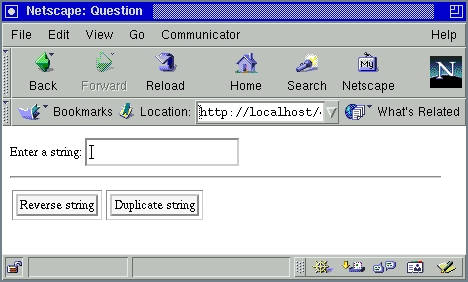
\includegraphics[scale=0.8]{PICTURES/revdup.jpg}
\end{center}\vspace{-3ex}
\caption{A simple string reverse/duplication form\label{fig-revdup}}
\end{figure}
%
\begin{prog}
rdForm :: IO HtmlForm
rdForm = return \$ form "Question"
           [htxt "Enter a string: ", textfield tref "", hrule,
            button "Reverse string"   revhandler,
            button "Duplicate string" duphandler]
 where
   tref free
~
   revhandler env = return \$ form "Answer"
     [h1 [htxt \$ "Reversed input: " ++ reverse (env tref)]]
~
   duphandler env = return \$ form "Answer"
     [h1 [htxt \$ "Duplicated input: " ++ env tref ++ env tref]]
\end{prog}
%
Note the simplicity of retrieving values entered into the form:
since the event handlers are called with the appropriate environment
containing these values (parameter \ccode{env}),
they can easily access these values
by applying the environment to the appropriate CGI reference,
like \ccode{(env tref)}.


\section{Further Examples for Web Server Programming}

Now we have seen all elements for writing CGI programs
in Curry.
In this section we will show by various examples how to use
this programming interface. We will see that this programming model
(i.e., logic variables for CGI references,
associated event handlers depending on CGI environments)
is sufficient to solve typical problems in web server programming
in an appropriate way, like
handling sequences of interactions or
holding intermediate states between interactions.


\subsection{Interaction Sequences}

In the previous example, the interaction between the
client and the web server is quite simple:
the client sends a request by filling a form which is answered
by the server with an HTML document containing the requested
information. In realistic applications, it is often the case
that the interaction is not finished by sending back the requested
information but the client requests further (e.g., more detailed)
information based on the received results. Thus, one
has to deal with sequences of longer interactions between the
client and the server.

Our programming model provides a direct support for
interaction sequences. Since the answer provided by the event handler
is an HTML form rather than an HTML expression,
this answer can also contain further input elements
and associated event handlers. By nesting event handlers,
it is straightforward to implement bounded sequences of interactions.
An example for this technique is shown in the next section.

A more interesting question is how to implement
other control abstractions like arbitrary loops.
For this purpose, we show the implementation of a simple
number guessing game: the client has to guess a number
known by the server (here: \code{42}), and for each number entered
by the client the server responds whether this number
is right, smaller or larger than the number to be guessed.
If the guess is not right, the answer form contains an input
field where the client can enter the next guess.
Moreover, the number of guesses should also be counted
and shown at the end.

As the typical approach in declarative languages,
we implement looping constructs by recursion.
Thus, the event handler computing the answer for the client
contains a recursive call to the initial form
which implements the interaction loop.
The entire implementation of this number guessing game
is as follows \proghref{guess}{Program}:
%
\begin{prog}
guessForm :: IO HtmlForm
guessForm = return \$ form "Number Guessing" (guessInput 1)
~
guessInput :: Int -> [HtmlExp]
guessInput n =
  [htxt "Guess a natural number: ", textfield nref "",
   button "Check" (guessHandler n nref)]   where nref free
~
guessHandler :: Int -> CgiRef -> (CgiRef -> String) -> IO HtmlForm
guessHandler n nref env =
  return \$ form "Answer" \$
    case reads (env nref) of
      [(nr,"")] ->
            if nr==42
              then [h1 [htxt \$ "Right! You needed "++show n++" guesses!"]]
              else [h1 [htxt \$ if nr<42 then "Too small!"
                                        else "Too large!"],
                    hrule] ++ guessInput (n+1)
      _ -> [h1 [htxt "Illegal input, try again!"]] ++ guessInput n
\end{prog}
%
\ccode{guessInput n} is an HTML expression corresponding to
the initial form which contains an
input field for entering the client's guess.
\ccode{guessHandler} is the associated event handler where the
number of guesses and the
CGI reference to the input field are the first and the second argument
of the handler, respectively.
It checks the number entered by the client
(\code{reads}\pindex{reads} is defined in the standard prelude
and used to parse a string into a value)
and returns the different answers depending on the client's guess.
If the guess is not right, the \code{guessInput} is appended
to the answer which implements the recursive call.


\subsection{Handling Intermediate States}
\label{sec-intermediate-state}

A nasty problem in many CGI applications is the handling
of intermediate states due to the fact that HTTP is a stateless
protocol. For instance, in electronic commerce applications,
the clients have shopping baskets where
the already selected items are stored, and the contents of
these baskets must be kept between the interactions.
Storing this information on the server side
has several drawbacks. For instance, the client
wants to identify himself only after he really orders
the items, i.e., during the selection phase the server
cannot uniquely associate the selections to a client.
Furthermore, the client might not proceed with his selections
so that the server does not know whether
the basket information can be deleted (which is necessary
at some point to avoid a memory overflow).
Therefore, it is often better to store such client-dependent
information on the client side. For this purpose,
one can have HTML forms with input elements of type \ccode{hidden}
which have no visual representation but can be used
to pass client-dependent information between interactions.
``Raw'' HTML/CGI programmers must explicitly handle
these fields which is awkward and a source of many
programming problems.

Our programming model offers a much simpler solution
to this problem. By nesting event handlers
(which is allowed in languages with lexical scoping like Curry),
one can directly refer to input elements in previous forms.
As a concrete example, we consider
a sequence of HTML forms where the client enters
his first name in the first form and his last name in the second form.
The complete name is returned in the third form.
This example can be implemented as follows
\proghref{state}{Program}:
%
\begin{prog}
nameForm = return \$ form "First Name Form"
  [htxt "Enter your first name: ", textfield firstref "",
   button "Continue" fhandler]
 where
   firstref free
~
   fhandler _ = return \$ form "Last Name Form"
                  [htxt "Enter your last name: ", textfield lastref "",
                   button "Continue" lhandler]
     where
       lastref free
~
       lhandler env = return \$ form "Answer"
                        [htxt \$ "Hi, " ++ env firstref ++ " " ++ env lastref]
\end{prog}
%
Due to lexical scoping, the variable \ccode{firstref}
is visible in the event handler \ccode{lhandler} without explicitly
passing it as an argument.


\subsection{Storing Information on the Server}

We have seen how we can retrieve information from the server
by CGI programs. This is possible by performing I/O actions
on the server before computing the HTML form as the response to
the client. In many applications, clients also want to store
or update information on the server, e.g., by putting orders
for books, flight tickets, etc.
In this section we will see a small example that demonstrates
how this can be done using the already known techniques.

Consider the implementation of a web form that counts
and shows the number of visitors. Thus, each visitor
updates the current visitor counter on the server.
This can be easily implemented by storing the current
visitor number in a file.
For this purpose, we define an I/O action \ccode{incVisitNumber}
that reads the number stored in this file, increments it,
stores the incremented number
in the file, and returns the incremented number
(\code{doesFileExist}\pindex{doesFileExist},
\code{removeFile}\pindex{removeFile}, and
\code{renameFile}\pindex{renameFile} are
I/O operations defined in the library \code{Directory}
to check the existence of a file, delete a file, and
rename a file, respectively):
%
\begin{prog}
incVisitNumber :: IO Int
incVisitNumber = do
 existnumfile <- doesFileExist visitFile
 if existnumfile
   then do vfcont <- readFile visitFile
           overwriteVisitFile (read vfcont + 1)
   else do writeFile visitFile "1"
           return 1
~
overwriteVisitFile :: Int -> IO Int\label{sec-overwriteVisitFile}
overwriteVisitFile n = do
  writeFile (visitFile++".new") (show n)
  removeFile visitFile
  renameFile (visitFile ++ ".new") visitFile
  return n
~
visitFile :: String
visitFile = "numvisit"  -- file to store the current visitor number
\end{prog}
%
Note the definition of \code{overwriteVisitFile}:
it does not directly write the incremented number
into the \code{visitFile} but it writes it into another file that is
subsequently renamed to the \code{visitFile}.
This is necessary to avoid the overlapping of reading and writing actions
on the same file due to the lazy evaluation of \code{readFile}.

Now the visitor form is simply obtained by calling \code{incVisitNumber}
before generating the form
\proghref{visitor}{Program}:
%
\begin{prog}
visitorForm = do
  visitnum <- incVisitNumber
  return \$ form "Access Count Form"
           [h1 [htxt \$ "You are the " ++ show visitnum ++ ". visitor!"]]
\end{prog}


\subsection{Ensuring Exclusive Access}
\label{sec-exclusiveIO}

Since CGI programs are executed whenever a client accesses them,
one has not much control on the order of their execution.
In particular, the same CGI program can be executed
in parallel if two clients accessing them simultaneously.
This can cause a problem if both update the same information.
For instance, an access to the visitor form above
reads the current visitor number from the global \code{visitFile}
and write the incremented number back.
If the script is simultaneously executed by two clients,
it may be the case that one update is lost (if both read the same
number and write the same incremented number).

Multiple simultaneous accesses or updates can be avoided
by ensuring the exclusive access to a resource on the web server
between different processes running on the server.
Although Curry has no direct features to support this,\footnote{%
It could be implemented in Curry by the use of ports but this
will be discussed later.}
it can be implemented by the use of the underlying
operating system. For instance, Unix/Linux systems
offer the command \ccode{lockfile} to ensure
an exclusive access to a resource of the system.
\code{lockfile} tries to create
a given file (the argument to \code{lockfile}).
If the file cannot be created (since it has been already created
by another process), the \code{lockfile} command waits
and retries after some time.
Using \code{lockfile}, we can implement a generic function
\ccode{exclusiveIO} that takes a name for a global lock file
and exclusively executes an I/O action (the second parameter),
i.e., it ensures that two processes using the same lock file
do not execute the action at the same time:
%
\begin{prog}
exclusiveIO :: String -> IO a -> IO a
exclusiveIO lockfile action = do
  system ("lockfile " ++ lockfile)
  actionResult <- action
  system ("rm -f " ++ lockfile)
  return actionResult
\end{prog}
%
Now it is straightforward to extend our visitor form
in order to ensure the exclusive update of the visitor counter.
This is done by replacing the expression \code{incVisitNumber}
in the definition of \code{visitorForm} by the following
expression \proghref{exclusive}{Program}:
%
\begin{prog}
exclusiveIO (visitFile ++ ".lock") incVisitNumber
\end{prog}


\subsection{Example: A Web Questionnaire}

\begin{figure}[t]
\begin{center}
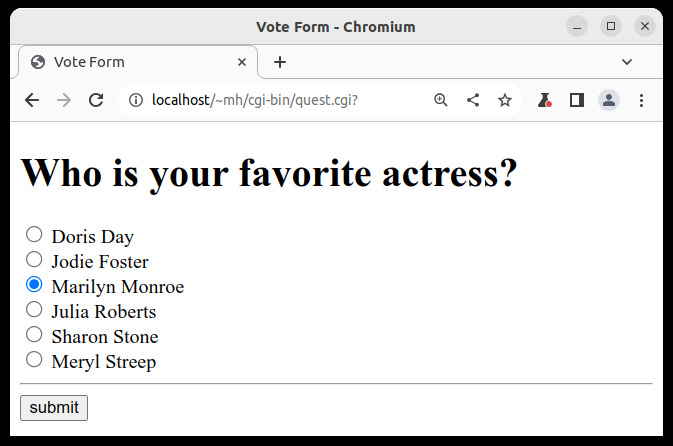
\includegraphics[scale=0.8]{PICTURES/quest.jpg}
\end{center}\vspace{-3ex}
\caption{A web questionnaire\label{fig-quest}}
\end{figure}

This section shows an example for web programming
where the formerly discussed techniques are applied.
Consider the implementation of a web-based questionnaire
which allows the clients to vote on a particular topic.
Figure~\ref{fig-quest} shows an example of such a questionnaire.
The votes are stored on the web server.
The current votings are shown after a client
submits a vote (see Figure~\ref{fig-quest-answer}).

\begin{figure}[t]
\begin{center}
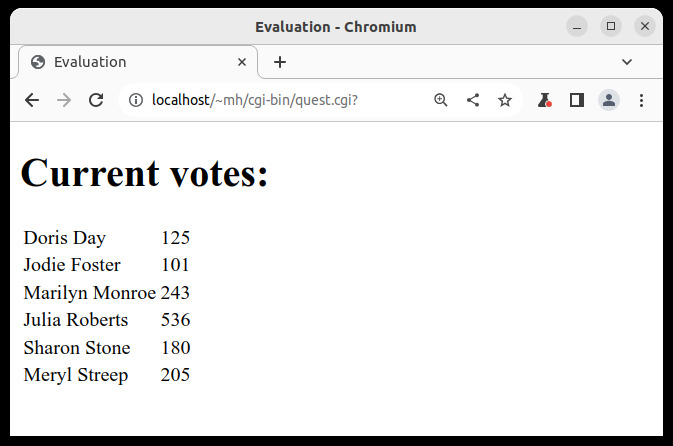
\includegraphics[scale=0.8]{PICTURES/quest_answer.jpg}
\end{center}\vspace{-3ex}
\caption{Answer to the web questionnaire\label{fig-quest-answer}}
\end{figure}

In order to provide an implementation that is easy to maintain,
we define the main question and the choices for the answers
as constants in our program so that they can be easily adapted
to other questionnaires:
\begin{prog}
question = "Who is your favorite actress?"
~
choices = ["Doris Day", "Jodie Foster", "Marilyn Monroe",
           "Julia Roberts", "Sharon Stone", "Meryl Streep"]
\end{prog}
%
The current votes are stored in a file on the web server.
We define the name of this file as a constant in our program:
%
\begin{prog}
voteFile = "votes.data"
\end{prog}
%
For the sake of simplicity, this file is a simple text file.
If there are $n$ choices for voting, the file has $n$ lines
where each line contains the textual representation of the
number of votes for the corresponding choice.
Thus, the following function defines an action that reads
the vote file and returns the list of numbers in this file
(the prelude function \code{lines}\pindex{lines} breaks
a string into a list of lines where lines are separated by newline
characters):
%
\begin{prog}
readVoteFile :: IO [Int]
readVoteFile = do
  vfcont <- readFile voteFile
  return (map read (lines vfcont))
\end{prog}
%
To initialize the vote file, we define an action \code{initVoteFile}
that initializes the vote file with \code{n} zeros if it does not exist.
The prelude function \code{unlines}\pindex{unlines}
is the opposite of \code{lines} and concatenates a list of strings
into one string by inserting newline characters.
%
\begin{prog}
initVoteFile :: Int -> IO ()
initVoteFile n = do
  existnumfile <- doesFileExist voteFile
  unless existnumfile \$
    writeFile voteFile (unlines (map show (take n (repeat 0))))
\end{prog}
%
To update the vote file, we define \code{overwriteVoteFile}
that writes a list of
numbers into the vote file. Similarly to the definition of
\code{overwriteVisitFile} in Section~\ref{sec-overwriteVisitFile},
the numbers are written into a new file that is moved to the vote file
in order to avoid an overlapping between reading and writing the same file.
%
\begin{prog}
overwriteVoteFile :: [Int] -> IO ()
overwriteVoteFile nums = do
  writeFile (voteFile ++ ".new") (unlines (map show nums))
  removeFile voteFile
  renameFile (voteFile ++ ".new") voteFile
\end{prog}
%
When a client submits a vote, we have to increment to corresponding
number in the vote file. This can be easily done by a sequence of
actions that initialize the vote file (if necessary), read the current
votes and write the votes that are incremented by the function
\code{incNth}:
\begin{prog}
incNumberInFile :: Int -> IO ()
incNumberInFile n = do
  initVoteFile (length choices)
  nums <- readVoteFile
  overwriteVoteFile (incNth nums n)
~
incNth :: [Int] -> Int -> [Int]
incNth []     _ = []
incNth (x:xs) n | n==0      = (x+1) : xs
                | otherwise = x : incNth xs (n-1)
\end{prog}
%
Now we have all auxiliary definitions that are necessary to define
the web script. First, we show the definition of
the HTML form \ccode{evalForm} that shows the current votes
(which produces the result shown in Figure~\ref{fig-quest-answer}).
Note that we ensure the exclusive access to the vote file
by the use of the function \ccode{exclusiveIO} defined in
Section~\ref{sec-exclusiveIO}
(the prelude function \ccode{zip}\pindex{zip} joins two lists
into one list of pairs of corresponding elements):
\begin{prog}
evalForm :: IO HtmlForm
evalForm = do
  votes <- exclusiveIO (voteFile ++ ".lock") readVoteFile
  return \$ form "Evaluation"
   [h1 [htxt "Current votes:"],
    table (map (\char92(s,v) -> [[htxt s], [htxt \$ show v]])
               (zip choices votes))]
\end{prog}
%
Now we can define our main form that allows the user to submit a
vote (see Figure~\ref{fig-quest}).
It uses radio buttons as input elements.
\label{radio button}\index{button!radio}
Radio buttons are lists of buttons where exactly one button
can be turned on. Thus, all buttons have the same CGI reference
but different values. When a form is submitted, the CGI environment
maps the CGI reference to the value of the selected radio button.
A complete radio button suite consists always of a main button
(\code{radio_main}) which is initially on and some further buttons
with the same CGI reference as the main button (\code{radio_others})
that are initially off.
In our example, we associate to each button the index of the corresponding
choice as a value. The event handler \code{questHandler}
increments he appropriate vote number and returns the current votes
with the form \code{evalForm}
\proghref{questionnaire}{Program}:
\begin{prog}
questForm = return \$ form "Vote Form" \$
  [h1 [htxt question],
   radio_main vref "0", htxt (' ':head choices), breakline] ++
  concatMap (\char92(i,s) -> [radio_other vref (show i), htxt (' ':s), breakline])
            (zip [1..] (tail choices)) ++
  [hrule, button "submit" questHandler]
 where
   vref free
~
   questHandler env = do
     exclusiveIO (voteFile ++ ".lock") (incNumberInFile (read (env vref)))
     evalForm
\end{prog}


\section{Finding Bugs}

Since debugging of CGI programs can be quite tedious,
here are some hints on how to debug CGI programs.

If the execution of the CGI program produces some run-time error
(e.g., access to a non-existing files), the error message
should be shown in the web page.
Furthermore, messages written to standard error output
are collected in the log file of the web script.
For instance, if the web script is stored at location
\code{cgi-bin/myscript.cgi},
the log file is \code{cgi-bin/myscript.cgi.log}.
Hence, if you want to put some debug output in your web script,
you should write it to standard error, e.g.,
%
\begin{prog}
hPutStrLn stderr "A log message"
\end{prog}
%
(where \code{hPutStrLn} and \code{stderr} are defined
in the standard library \code{IO}).

% If the execution of the CGI program does not produce a run-time error
% but simply fails (e.g., because of an incompletely defined function
% are a unification failure), you will probably see the message
% \ccode{No more solutions} in the web browser instead of the
% expected HTML document. For the purpose of debugging,
% it is often useful to see the subexpressions where a
% reduction was not possible but failed. In this case,
% you can  generate the CGI program by \ccode{makecurrycgi}\pindex{makecurrycgi}
% with the option \ccode{-debug}.
% This has the effect that some debugging code is inserted in the CGI
% program so that you can see the trace of all failed subexpressions
% in the browser (not formatted with HTML so that you should better
% view the source with your browser). Note that the debug option
% produces less efficient CGI programs so that it is better to
% use this option only when necessary.

The use of logic variables as references to input elements
in HTML forms ensures that typos in the name of references
can be detected by the compiler (e.g., resulting in an
``undeclared identifier'' error message), in contrast
to traditional approaches to CGI programming using plain strings
as references.
However, if we use the same logic variable for two different
input elements, this is not detected by the compiler
(which is not worse than traditional approaches where this
is also not detected) but results in a run-time error
that is not easy to understand due to the implementation
of the library \code{HTML.Base} in Curry.
In this case, the web script might fail with a message like
\ccode{No value found}.
Thus, you should check your source program for these possible errors
or add some debug output, as described above, to your script.


\section{Advanced Web Programming}
\label{sec-advanced-web-programming}

This section discusses some further features which are useful
for writing web applications in Curry.
\emph{Cookies} are useful to store information about the client
between different web scripts.
\emph{URL parameters} can be exploited to write generic web scripts.
\emph{Style sheets} can be used to modify and add new presentation styles
for web documents.


\subsection{Cookies}

Cookies\index{cookie} are small pieces of information
(represented by strings) that are stored on the client's machine
when a client communicates to a web server via his browser.
The web server can sent cookies to the client together
with a requested web document. If the client wants to retrieve
the same or another document from the web server, the client's browser
sends the stored cookies together with the request for a document
to the browser.
Thus, cookies can be used to identify the client during a longer
interaction with the web server (also across various web scripts
stored on the same web browser).
Cookies are another approach to handle intermediate state
in web applications. The technique presented in
Section~\ref{sec-intermediate-state} is only useful
inside the same web script whereas cookies can be used
as a link between different web scripts.
However, cookies need special support on the browser's side
and the client must enable cookies in his web browser.
Fortunately, most web browsers support cookies
since they are used in many web sites.

Basically, a cookie has a name and a value.
Both parameters are of type string.
Cookies can also have additional parameters to control their
lifetime, validity for different web servers or regions
on a web server etc (see definition of datatype
\ccode{CookieParam} in the library \code{HTML.Base}) which we will not describe
here. As the default, a cookie is a valid during the client's
browser session for all documents in the same directory or
a subdirectory in which the cookie was set.

The library \code{HTML.Base} provides two functions to set
and retrieve cookies.
As described above, a cookie is set by sending it with some
web document. For doing so, there is the function
%
\begin{prog}
cookieForm :: String -> [(String,String)] -> [HtmlExp] -> HtmlForm\pindex{cookieForm}
\end{prog}
%
which behaves similarly to the function \ccode{form} but
takes an additional parameter: a list of cookies, i.e.,
name/value pairs. These cookies are submitted with the form
to the client's browser. To retrieve cookies (that are previously sent
with a \ccode{cookieForm}), there is an I/O action
%
\begin{prog}
getCookies :: IO [(String,String)]\pindex{getCookies}
\end{prog}
%
that returns the list of all cookies (i.e., name/value pairs)
sent from the browser for the current CGI script.

As a simple example, we want to use cookies to write a web application
where a user must identify himself and this identification is used
in another independent script. The identification is done
by setting a cookie of the form \code{("LOGINNAME",<name>)}
where \code{<name>} is the user's name.
We implement a ``login form'' that sets this cookie as follows
\proghref{logincookie}{Program}:
\begin{prog}
loginForm = return \$ form "Login"
  [htxt "Enter your name: ", textfield tref "",
   hrule,
   button "Login" handler
  ]
 where
   tref free
~
   handler env = return \$
     cookieForm "Logged In"
                [("LOGINNAME",env tref)]
                [h2 [htxt \$ env tref ++ ": thank you for visiting us"]]
\end{prog}
The first form asks the user for his name.
The cookie is set together with the acknowledgment form
(function \ccode{handler}).

Now we can write another web script that uses this cookie.
This script shows the user's name or the string
\code{"Not yet logged in"} if the user has not used the
login form to set the cookie.
Using the function \code{getCookies}, the implementation
is quite simple (the function \code{lookup}\pindex{lookup}, defined in the
prelude, searches for a name in a name/value list;
it returns \ccode{Nothing} of the name was not found and
\ccode{Just v} if the first occurrence of the name in the list
has the associated value \code{v}; the prelude function
\code{maybe}\pindex{maybe} processes these two cases)
\proghref{logincookie}{Program}:
\begin{prog}
getNameForm = do
  cookies <- getCookies
  return \$ form "Hello" \$
   maybe [h1 [htxt "Not yet logged in"]]
         (\char92n->[h1 [htxt \$ "Hello, " ++ n]])
         (lookup "LOGINNAME" cookies)
\end{prog}
%
As mentioned above, cookies need special support on the client's
side, i.e., the web browser of the client must support cookies.
If cookies are essential for an application, one should check
whether the client allows the setting of cookies.
This can be done by trying to set a cookie and by checking
whether this was successful. For instance, one can modify
the above login script as folllows.
The first form immediately sets a cookie with name \ccode{SETCOOKIE}.
Then the handler checks whether this cookie has been sent by the
client's browser. If this cookie is not received, it returns a form
with the message ``Sorry, can't set cookies.'' instead of the
acknowledgment form which sets the cookie \ccode{LOGINNAME}
\proghref{checkcookie}{Program}:
\begin{prog}
loginForm = return \$ cookieForm "Login" [("SETCOOKIE","")]
  [htxt "Enter your name: ", textfield tref "",
   hrule,
   button "Login" handler
  ]
 where
   tref free
~
   handler env = do
     cookies <- getCookies
     return \$
       if lookup "SETCOOKIE" cookies == Nothing
       then form "No cookies" [h2 [htxt "Sorry, can't set cookies."]]
       else cookieForm "Logged In"
                       [("LOGINNAME", env tref)]
                       [h2 [htxt \$ env tref ++ ": thank you for visiting us"]]
\end{prog}


\subsection{URL Parameters}

In some situations it is preferable to have generic web scripts that
can be applied in various situations described by parameters.
For instance, if we want to write a web application that
allows the navigation through a hierarchical structure,
one does not want to write a different script for each different
level of the structure but it is preferable to write a single
script that can be applied to different points in the structure.
This is possible by attaching a parameter (a string)
to the URL of a script. For instance, a URL can have the form
\ccode{http://myhost/script.cgi?parameter} where
\ccode{http://myhost/script.cgi} is the URL of the web script
and \ccode{parameter} is an optional parameter that is passed
to the script.
A \emph{URL parameter}\index{URL!parameter}\index{parameter!URL}
can be retrieved inside a script
by the I/O action
%
\begin{prog}
getUrlParameter :: IO String \pindex{getUrlParameter}
\end{prog}
%
which returns the part of the URL following the character \ccode{?}.
Note that an URL parameter should be ``URL encoded'' to avoid
the appearance of characters with a special meaning.
The library \code{HTML.Base} provides the functions
\code{urlencoded2string} and \code{string2urlencoded}
to decode and encode such parameters, respectively.

As a simple example, we want to write a web script to navigate
through a directory structure. The current directory
is the URL parameter for this script. The script
extracts this parameter by the use of \code{getUrlParameter}
and shows all entries as a HTML list
\proghref{browsedir}{Program}
(the prelude function \code{mapM}\pindex{mapM} applies
a mapping from elements into actions to all elements of a list
and collect all results in a list):
%
\begin{prog}
showDirForm = do
  param <- getUrlParameter
  let dir = if param=="" then "." else urlencoded2string param
  entries <- getDirectoryContents dir
  hexps <- mapM (entry2html dir) entries
  return \$ form "Browse Directory"
                [h1 [htxt \$ "Directory: " ++ dir], ulist hexps]
\end{prog}
%
The I/O action \code{getDirectoryContents}\pindex{getDirectoryContents}
is defined in the system library \code{Directory}
and returns the list of all entries in a directory.
The function \code{entry2html} checks for an entry whether it
is a directory. If this is the case, it returns a link to
the same web script but with an extended parameter, otherwise
it simply returns the entry name as an HTML text
(\code{doesDirectoryExist}\pindex{doesDirectoryExist}
is defined in the library \code{Directory} and returns \code{True}
if the argument is the name of a directory):
%
\begin{prog}
entry2html :: String -> String -> IO [HtmlExp]
entry2html dir e = do
  direx <- doesDirectoryExist (dir ++ "/" ++ e)
  if direx
   then return [href ("browsedir.cgi?" ++ string2urlencoded (dir ++ "/" ++ e))
                     [htxt e]]
   else return [htxt e]
\end{prog}
%


\subsection{Style Sheets}

\todo{To be completed.}


%%% Local Variables: 
%%% mode: latex
%%% TeX-master: "main"
%%% End: 
% LocalWords:  HTML CGI URL

\chapter{Further Libraries for Application Programming}

\begin{itemize}
\item Databases \cite{Hanus04JFLP}
\item Constraints
\item GUI \cite{Hanus00PADL}
\item XML
\item Distributed Programming, ports \cite{Hanus99PPDP}
\item Metaprogramming
\end{itemize}


%%% Local Variables: 
%%% mode: latex
%%% TeX-master: "main"
%%% End: 


\newpage
\addcontentsline{toc}{chapter}{Bibliography}
\bibliography{biblio}
\bibliographystyle{abbrv}

\newpage
\addcontentsline{toc}{chapter}{Index}
\printindex

\end{document}
